	%%  A simple AAU report template.

%  2014-09-13 v. 1.1.0
%  Copyright 2010-2014 by Jesper Kjær Nielsen <jkn@es.aau.dk>
%
%  This is free software: you can redistribute it and/or modify
%  it under the terms of the GNU General Public License as published by
	%  the Free Software Foundation, either version 3 of the License, or
%  (at your option) any later version.
%
%  This is distributed in the hope that it will be useful,
%  but WITHOUT ANY WARRANTY; without even the implied warranty of
%  MERCHANTABILITY or FITNESS FOR A PARTICULAR PURPOSE.  See the
%  GNU General Public License for more details.
%
%  You can find the GNU General Public License at <http://www.gnu.org/licenses/>.
%
%  A simple AAU report template.
%  2014-09-13 v. 1.1.0
%  Copyright 2010-2014 by Jesper Kjær Nielsen <jkn@es.aau.dk>
%
%  This is free software: you can redistribute it and/or modify
%  it under the terms of the GNU General Public License as published by
%  the Free Software Foundation, either version 3 of the License, or
%  (at your option) any later version.
%
%  This is distributed in the hope that it will be useful,
%  but WITHOUT ANY WARRANTY; without even the implied warranty of
%  MERCHANTABILITY or FITNESS FOR A PARTICULAR PURPOSE.  See the
%  GNU General Public License for more details.
%
%  You can find the GNU General Public License at <http://www.gnu.org/licenses/>.
%
\documentclass[11pt,twoside,a4paper,openright]{report}
%%%%%%%%%%%%%%%%%%%%%%%%%%%%%%%%%%%%%%%%%%%%%%%%
% Language, Encoding and Fonts
% http://en.wikibooks.org/wiki/LaTeX/Internationalization
%%%%%%%%%%%%%%%%%%%%%%%%%%%%%%%%%%%%%%%%%%%%%%%%
% Select encoding of your inputs. Depends on
% your operating system and its default input
% encoding. Typically, you should use
%   Linux  : utf8 (most modern Linux distributions)
%            latin1 
%   Windows: ansinew
%            latin1 (works in most cases)
%   Mac    : applemac
% Notice that you can manually change the input
% encoding of your files by selecting "save as"
% an select the desired input encoding. 
\usepackage[utf8]{inputenc}
% Make latex understand and use the typographic
% rules of the language used in the document.
\usepackage[danish,english]{babel}
% Use the vector font Latin Modern which is going
% to be the default font in latex in the future.
\usepackage{lmodern}
% Choose the font encoding
\usepackage[T1]{fontenc}
% For checkmarks: \cmark and crossmarks: \xmark
\usepackage{pifont}
	\newcommand{\cmark}{\ding{51}}%
	\newcommand{\xmark}{\ding{55}}%
%%%%%%%%%%%%%%%%%%%%%%%%%%%%%%%%%%%%%%%%%%%%%%%%
% Graphics and Tables
% http://en.wikibooks.org/wiki/LaTeX/Importing_Graphics
% http://en.wikibooks.org/wiki/LaTeX/Tables
% http://en.wikibooks.org/wiki/LaTeX/Colors
%%%%%%%%%%%%%%%%%%%%%%%%%%%%%%%%%%%%%%%%%%%%%%%%
% load a colour package
\usepackage[table,dvipsnames]{xcolor}
\definecolor{aaublue}{RGB}{33,26,82}% dark blue
\definecolor{lightGrey}{RGB}{240,240,240}% 
% The standard graphics inclusion package
\usepackage{graphicx}
% Load package to convert eps-files to use as figures
\usepackage{epstopdf}

%\usepackage[dvips,final]{graphicx} 
%\usepackage[dvips]{geometry}
\usepackage{color} %include even if images aren’t in color \usepackage{epsfig}
\usepackage{latexsym}
\usepackage{pstricks}

%\usepackage{epsfig}

% Set up how figure and table captions are displayed
\usepackage{caption}
\captionsetup{%
  font=footnotesize,% set font size to footnotesize
  labelfont=bf % bold label (e.g., Figure 3.2) font
}
\usepackage[section]{placeins} % Figurer overskrider ikke sections
% For subfigures
\usepackage{subcaption}
% Make the standard latex tables look so much better
\usepackage{array,booktabs}
% Enable the use of frames around, e.g., theorems
% The framed package is used in the example environment
\usepackage{framed}

% Afstand mellem listepunkter og tilføjelse af resume funktion til lister: \begin{enumerate}[resume]
\usepackage{enumitem}
\setlist{itemsep=-2pt}

% Tilføjer mulighed for at lave enkelte sider i landskab.
\usepackage{lscape}

\newcounter{listcounter}
%%%%%%%%%%%%%%%%%%%%%%%%%%%%%%%%%%%%%%%%%%%%%%%%
% Mathematics
% http://en.wikibooks.org/wiki/LaTeX/Mathematics
%%%%%%%%%%%%%%%%%%%%%%%%%%%%%%%%%%%%%%%%%%%%%%%%
% Defines new environments such as equation,
% align and split 
\usepackage{amsmath}
% Adds new math symbols
\usepackage{amssymb}
% Use theorems in your document
% The ntheorem package is also used for the example environment
% When using thmmarks, amsmath must be an option as well. Otherwise \eqref doesn't work anymore.
\usepackage[framed,amsmath,thmmarks]{ntheorem}

% Tilføjer \degree symbol
\usepackage{textcomp}
\usepackage{gensymb}

% Fjerner mellemrum efter komma i formler.
%\usepackage{icomma}

% Packages for SI units
\usepackage[binary-units]{siunitx}
% Format SI units as italic in italic texts
\sisetup{detect-all}
\sisetup{per-mode=symbol}


% Argument til amsmath der gør parenteser uden om parenteser pænere ved brug af \right og \left kommandoerne
\delimitershortfall=-1pt

%%%%%%%%%%%%%%%%%%%%%%%%%%%%%%%%%%%%%%%%%%%%%%%%
% Page Layout
% http://en.wikibooks.org/wiki/LaTeX/Page_Layout
%%%%%%%%%%%%%%%%%%%%%%%%%%%%%%%%%%%%%%%%%%%%%%%%
% Change margins, papersize, etc of the document
\usepackage[
  inner=28mm,% left margin on an odd page
  outer=41mm,% right margin on an odd page
  ]{geometry}
% Modify how \chapter, \section, etc. look
% The titlesec package is very configureable
\usepackage[explicit]{titlesec}
%\titleformat*{\section}{\normalfont\Large\bfseries\color{aaublue}}
%\titleformat*{\subsection}{\normalfont\large\bfseries\color{aaublue}}
%\titleformat*{\subsubsection}{\normalfont\normalsize\bfseries\color{aaublue}}
%\titleformat*{\paragraph}{\normalfont\normalsize\bfseries\color{aaublue}}
%\titleformat*{\subparagraph}{\normalfont\normalsize\bfseries\color{aaublue}}
\usepackage{calc}

% Spacing omkring kapiteloverskrift
\titlespacing*{\chapter}{0pt}{40pt}{50pt}



% Overskrift med stort nummer til venstre og titel til højre
%\newlength\chapnumb
%\setlength{\chapnumb}{1.5cm}
%\titleformat{\chapter}[block]
%{\normalfont\bfseries}{}{0pt}
%{\parbox[b]{\chapnumb}{%
	  %\fontsize{2cm}{0}\selectfont\thechapter}%
  %\parbox[b]{\dimexpr\textwidth-\chapnumb\relax}{%
    %\raggedleft%
    %\hfill{\Huge#1}\\
    %\rule{\dimexpr\textwidth-\chapnumb\relax}{.5pt}}}
%\titleformat{name=\chapter,numberless}[block]
%{\normalfont\bfseries}{}{0pt}
	%{\Huge#1}

% Clear empty pages between chapters
\let\origdoublepage\cleardoublepage
\newcommand{\clearemptydoublepage}{%
  \clearpage
  {\pagestyle{empty}\origdoublepage}%
}
\let\cleardoublepage\clearemptydoublepage

% Change the headers and footers
\usepackage{fancyhdr}
\pagestyle{fancy}
\fancyhf{} %delete everything
\renewcommand{\headrulewidth}{0pt} %remove the horizontal line in the header
\fancyhead[RE]{\color{black}\small\nouppercase\leftmark} %even page - chapter title
\fancyhead[LO]{\color{black}\small\nouppercase\rightmark} %uneven page - section title
\fancyhead[LE,RO]{\thepage} %page number on all pages
% Do not stretch the content of a page. Instead,
% insert white space at the bottom of the page
\raggedbottom
% Enable arithmetics with length. Useful when
% typesetting the layout.

\setlength{\headheight}{14pt}

% Raise penalties for bastards
\widowpenalty=10000
\clubpenalty=10000

%%%%%%%%%%%%%%%%%%%%%%%%%%%%%%%%%%%%%%%%%%%%%%%%
% Table of Contents
% http://en.wikibooks.org/wiki/LaTeX/Bibliography_Management
%%%%%%%%%%%%%%%%%%%%%%%%%%%%%%%%%%%%%%%%%%%%%%%%
% Add additional commands for Table of Contents
\usepackage{bookmark}

{\setcounter{tocdepth}{1}}

% Control of space between items in Table of Contents
\usepackage[titles]{tocloft}
\setlength{\cftbeforepartskip}{10pt}
\setlength{\cftbeforechapskip}{4pt}
\setlength{\cftbeforesecskip}{2pt}
%%%%%%%%%%%%%%%%%%%%%%%%%%%%%%%%%%%%%%%%%%%%%%%%
% Bibliography
% http://en.wikibooks.org/wiki/LaTeX/Bibliography_Management
%%%%%%%%%%%%%%%%%%%%%%%%%%%%%%%%%%%%%%%%%%%%%%%%
% Add the \citep{key} command which display a
% reference as [author, year]
\usepackage[square]{natbib}

%%%%%%%%%%%%%%%%%%%%%%%%%%%%%%%%%%%%%%%%%%%%%%%%
% Misc
%%%%%%%%%%%%%%%%%%%%%%%%%%%%%%%%%%%%%%%%%%%%%%%%
% Add bibliography and index to the table of
% contents
\usepackage[nottoc]{tocbibind}
% Add the command \pageref{LastPage} which refers to the
% page number of the last page
\usepackage{lastpage}
\usepackage[
%  disable, %turn off todonotes
  colorinlistoftodos, %enable a coloured square in the list of todos
  textwidth=\marginparwidth, %set the width of the todonotes
  textsize=scriptsize, %size of the text in the todonotes
  ]{todonotes}

% Add command \includepdf to add a whole pdf page to document
\usepackage{pdfpages}


% Add option to easy format directory tree
\usepackage{dirtree}

% String manipulation
\usepackage{xstring,xifthen}

% Tikz package for drawing nice figures
\usepackage{tikz}
\usepackage{schemabloc}
\usetikzlibrary{circuits}


% Package for drawing pretty schematics, without leaving LaTex
\usepackage[american currents, american voltages, european resistors, cute inductors,
american ports]{circuitikz}
\usepackage{tikzscale}

% Code syntax highlight
\usepackage{listings}
\lstset{breaklines=true,
		breakatwhitespace=true,
		commentstyle=\color{ForestGreen},
		numbers=left,
		numberstyle=\tiny\color{black},
		keywordstyle=\color{blue},
		basicstyle=\footnotesize\ttfamily,
        showstringspaces=false,
		}
\renewcommand{\lstlistingname}{Code Snippet}

%%%%%%%%%%%%%%%%%%%%%%%%%%%%%%%%%%%%%%%%%%%%%%%%
% Table environments
% http://en.wikibooks.org/wiki/LaTeX/Tables
%%%%%%%%%%%%%%%%%%%%%%%%%%%%%%%%%%%%%%%%%%%%%%%%
% Better table environments for stuff like table width specifier
\usepackage{tabularx}
\usepackage{multirow}
\usepackage{longtable}
%%%%%%%%%%%%%%%%%%%%%%%%%%%%%%%%%%%%%%%%%%%%%%%%
% Project info and abstract
% chapters\abstract.tex, chapters\projectinfo.tex
%%%%%%%%%%%%%%%%%%%%%%%%%%%%%%%%%%%%%%%%%%%%%%%%
% Loads project info and abstract for use in
% hypersetup
\newcommand{\projectFaculty}{%
\iflanguage{english}{%
Vision, Graphics and Interactive Systems%
}{%
Vision, Grafik og Interaktive Systemer%
}}

\newcommand{\projectGroup}{%
\iflanguage{english}{%
Group 18gr842%
}{%
Gruppe 18gr842%
}}

\newcommand{\projectSemester}{%
P8%
}

\newcommand{\projectType}{%
\iflanguage{english}{%
Project Report%
}{%
Projektrapport%
}}

\newcommand{\projectTitle}{%
\iflanguage{english}{%
Noget med Computer Vision%
}{%
Noget med Computer Vision%
}}

\newcommand{\projectSubtitle}{%
\iflanguage{english}{%
- Subtitle -%
}{%
- Undertitel -%
}}

\newcommand{\projectTheme}{%
\iflanguage{english}{%
Computer Vision%
}{%
Computer Vision%
}}

\newcommand{\projectPeriod}{%
\iflanguage{english}{%
Spring Semester 2018%
}{%
Forårssemester 2018%
}}



\newcommand{\projectParticipants}{%
Marike Koch van den Broek\\
Shagen Djanian\\
Niclas Hjorth Stjernholm
}

\newcommand{\projectSupervisors}{%
Kamal Nasrollahi
}

\newcommand{\projectCopies}{8}

\newcommand{\projectCompletion}{
\iflanguage{english}{%
May 30, 2018%
}{
30. maj 2018%
}}




\newcommand{\projectAbstract}{
%Write the abstract here 
}

\newcommand{\projectSynopsis}{
Synopsis
}

%%%%%%%%%%%%%%%%%%%%%%%%%%%%%%%%%%%%%%%%%%%%%%%%
% Hyperlinks
% http://en.wikibooks.org/wiki/LaTeX/Hyperlinks
%%%%%%%%%%%%%%%%%%%%%%%%%%%%%%%%%%%%%%%%%%%%%%%%
% Enable hyperlinks and insert info into the pdf
% file. Hypperref should be loaded as one of the 
% last packages
\usepackage{hyperref}
\hypersetup{%
	%pdfpagelabels=true,%
	plainpages=false,%
	pdfauthor={\projectGroup, \projectFaculty, \iflanguage{english}{Aalborg University}{Aalborg Universitet}},%
	pdftitle={\projectTitle},%
	pdfsubject={\projectTheme},%
	bookmarksnumbered=true,%
	colorlinks,%
	citecolor=black,%aaublue,%
	filecolor=black,%aaublue,%
	linkcolor=black,%aaublue,% you should probably change this to black before printing
	urlcolor=black,%aaublue,%
	pdfstartview=FitH,%
	bookmarksdepth=2,%
}

% Defines where URLs should break
\def\UrlBreaks{\do\/\do-\do_}
\urlstyle{same}

% Give the possibility to autoformat reference based on distance to the referenced page. Ex. \vpageref{}
\usepackage{varioref}


% Package to warn about missing references.
%\usepackage{refcheck}

% Package to make a glossary of acronyms.
\usepackage{glossaries}
\glstoctrue
\makenoidxglossaries
% Glossaries package
% http://ctan.cs.uu.nl/macros/latex/contrib/glossaries/glossariesbegin.pdf
%
% % % % % % % %
%	Example of glossary entry:
% \newglossaryentry{cabbage}{name={cabbage},description={vegetable with thick green or purple leaves}}
%
%	Example of acronym entry:
% \newacronym{spi}{SPI}{Serial Peripheral Interface}
%
% \gls{key}

\newacronym{cdf}{CDF}{Cumulative Distribution Function}
\newacronym{cnn}{CNN}{Convolutional Neural Network}
\newacronym{cpu}{CPU}{Central Processing Unit}
\newacronym{fcn}{FCN}{Fully Convolutional Network}
\newacronym{dbn}{DBN}{Deep Belief Network}
\newacronym{deepid}{DeepID}{Deep hidden identity features}
\newacronym{deepid2}{DeepID2}{Deep IDentification-verification features}
\newacronym{gpu}{GPU}{Graphics Processing Unit}
\newacronym{spdnn}{SPDNN}{Semi Parallel Deep Neural Networks}
\newacronym{lfw}{LFW}{Labeled Faces in the Wild}
\newacronym{hmm}{HMM}{Hidden Markov Model}
\newacronym{lda}{LDA}{Linear Discriminant Analysis}
\newacronym{pca}{PCA}{Principal Component Analysis}
\newacronym{svm}{SVM}{support vector machines}
\newacronym{knn}{KNN}{K-Nearest-Neighbours}
\newacronym{vl}{VL}{Visible Light}
\newacronym{nir}{NIR}{Near Infra-Red}
\newacronym{mcs}{MCS}{Multiple Classifier Systems}
\newacronym{relu}{ReLU}{Rectified Linear Unit}
\newacronym{fc}{FC}{Fully Connected}


% Package to make semi-bold font.
\usepackage[outline]{contour}
\contourlength{0.1pt}
\contournumber{50}%
\newcommand{\textsb}[1]{\contour{black}{#1}}

% Package for splitting lists or other things up in columns. Ex: \begin{multicols}{2}
\usepackage{multicol}

% Package for rotating a page to landscape orientation. Ex: \begin{landscape}
\usepackage{pdflscape}

% Package for circuit diagrams in tikz
\usepackage{circuitikz}

% For adding notes to tables
\usepackage{threeparttable}

% For adding smileys ;) I know....
\usepackage{MnSymbol,wasysym}

% For adding algorithms
\usepackage{algorithm}
\usepackage[noend]{algpseudocode}
\makeatletter
\def\BState{\State\hskip-\ALG@thistlm}
\makeatother

\renewcommand*{\glsgroupskip}{\vspace{2mm}}

% Package to use fixme fxnote
\usepackage[footnote,marginclue,draft,danish,silent,nomargin]{fixme} 

% Package inclusion and set up of the document

% see, e.g., http://en.wikibooks.org/wiki/LaTeX/Formatting#Hyphenation
% for more information on word hyphenation
\hyphenation{ex-am-ple hy-phen-a-tion short}
\hyphenation{long la-tex}
\hyphenation{AAU-Sat}
\hyphenation{minimum-spændinger}
\hyphenation{ud-vik-lings-poten-tiale}
\hyphenation{pick-up pick-up-pen gui-tar-pick-up gui-tar-pick-up-pen pick-uppens}
\hyphenation{tech-no-lo-gy}
\hyphenation{Hø-re-for-e-ning-en}% Hypenation setup

%  A simple AAU report template.
%  2014-09-13 v. 1.1.0
%  Copyright 2010-2014 by Jesper Kjær Nielsen <jkn@es.aau.dk>
%
%  This is free software: you can redistribute it and/or modify
%  it under the terms of the GNU General Public License as published by
%  the Free Software Foundation, either version 3 of the License, or
%  (at your option) any later version.
%
%  This is distributed in the hope that it will be useful,
%  but WITHOUT ANY WARRANTY; without even the implied warranty of
%  MERCHANTABILITY or FITNESS FOR A PARTICULAR PURPOSE.  See the
%  GNU General Public License for more details.
%
%  You can find the GNU General Public License at <http://www.gnu.org/licenses/>.
%
%
%
% see, e.g., http://en.wikibooks.org/wiki/LaTeX/Customizing_LaTeX#New_commands
% for more information on how to create macros

%%%%%%%%%%%%%%%%%%%%%%%%%%%%%%%%%%%%%%%%%%%%%%%%
% Loads user defined variables
%%%%%%%%%%%%%%%%%%%%%%%%%%%%%%%%%%%%%%%%%%%%%%%%

\newcommand{\noSIunit}{$1$}% Definerer hvad der skal skrives hvis symbolet ikke har nogen enhed.
\newcommand{\obcTransducerAddress}{0xB1}% CAN adresse til tranducer modulet i OBC.

\def\circuitScale{.5}%

%%%%%%%%%%%%%%%%%%%%%%%%%%%%%%%%%%%%%%%%%%%%%%%%
% Macros for the titlepage
%%%%%%%%%%%%%%%%%%%%%%%%%%%%%%%%%%%%%%%%%%%%%%%%
%Creates the aau titlepage
\newcommand{\aautitlepage}[3]{%
  {
    %set up various length
    \ifx\titlepageleftcolumnwidth\undefined
      \newlength{\titlepageleftcolumnwidth}
      \newlength{\titlepagerightcolumnwidth}
    \fi
    \setlength{\titlepageleftcolumnwidth}{0.5\textwidth-\tabcolsep}
    \setlength{\titlepagerightcolumnwidth}{\textwidth-2\tabcolsep-\titlepageleftcolumnwidth}
    %create title page
    \thispagestyle{empty}
    \noindent%
    \begin{tabular}{@{}ll@{}}
      \parbox{\titlepageleftcolumnwidth}{
        \iflanguage{danish}{%
          
\includegraphics[page=1,width=\titlepageleftcolumnwidth]{figures/aau_logo}
        }{%
          
\includegraphics[page=2,width=\titlepageleftcolumnwidth]{figures/aau_logo}
        }
      } &
      \parbox{\titlepagerightcolumnwidth}{\raggedleft\sf\small
        #2
      }\bigskip\\
       #1 &
      \parbox[t]{\titlepagerightcolumnwidth}{%
        \iflanguage{danish}{%
          \textbf{Synopsis:}\smallskip\par
        }{%
          \textbf{Abstract:}\smallskip\par
        }
        \fbox{\parbox{\titlepagerightcolumnwidth-2\fboxsep-2\fboxrule}{%
          #3
        }}
      }\\
    \end{tabular}
    \vfill
    \iflanguage{danish}{%
      \noindent{\footnotesize\emph{Rapportens indhold er frit tilgængeligt, men offentliggørelse (med kildeangivelse) må kun ske efter aftale med forfatterne.}}
    }{%
      \noindent{\footnotesize\emph{The content of this report is freely available, but publication may only be pursued with reference.}}
    }
    \cleardoublepage
  }
}

%Create english project info
\newcommand{\englishprojectinfo}[8]{%
  \parbox[t]{\titlepageleftcolumnwidth}{
    \textbf{Title:}\\ #1\bigskip\par
    \textbf{Theme:}\\ #2\bigskip\par
    \textbf{Project Period:}\\ #3\bigskip\par
    \textbf{Project Group:}\\ #4\bigskip\par
    \textbf{Participants:}\\ #5\bigskip\par
    \textbf{Supervisor:}\\ #6\bigskip\par
    \textbf{Number of Pages:} \pageref{LastPage}\bigskip\par
    \textbf{Date of Completion:}\\ #8
  }
}

%Create danish project info
\newcommand{\danishprojectinfo}[8]{%
  \parbox[t]{\titlepageleftcolumnwidth}{
    \textbf{Titel:}\\ #1\bigskip\par
    \textbf{Tema:}\\ #2\bigskip\par
    \textbf{Projektperiode:}\\ #3\bigskip\par
    \textbf{Projektgruppe:}\\ #4\bigskip\par
    \textbf{Deltagere:}\\ #5\bigskip\par
    \textbf{Vejleder:}\\ #6\bigskip\par
    \textbf{Oplagstal:} #7\bigskip\par
    \textbf{Sidetal:} \pageref{LastPage}\bigskip\par
    \textbf{Afleveringsdato:}\\ #8
  }
}

%%%%%%%%%%%%%%%%%%%%%%%%%%%%%%%%%%%%%%%%%%%%%%%%
% An example environment
%%%%%%%%%%%%%%%%%%%%%%%%%%%%%%%%%%%%%%%%%%%%%%%%
\theoremheaderfont{\normalfont\bfseries}
\theorembodyfont{\normalfont}
\theoremstyle{break}
\def\theoremframecommand{{\color{aaublue!50}\vrule width 5pt \hspace{5pt}}}
\newshadedtheorem{exa}{Example}[chapter]
\newenvironment{example}[1]{%
		\begin{exa}[#1]
}{%
		\end{exa}
}


%%%%%%%%%%%%%%%%%%%%%%%%%%%%%%%%%%%%%%%%%%%%%%%%%
% Exponential function defined as upright e, \exp
%%%%%%%%%%%%%%%%%%%%%%%%%%%%%%%%%%%%%%%%%%%%%%%%%
\renewcommand{\exp}{\text{e}}


%%%%%%%%%%%%%%%%%%%%%%%%%%%%%%%%%%%%%%%%%%%%%%%%%%%
% Command \clearevenpage start chapter on even page
%%%%%%%%%%%%%%%%%%%%%%%%%%%%%%%%%%%%%%%%%%%%%%%%%%%
\makeatletter
\newcommand*{\clearevenpage}{%
  \clearpage
  \if@twoside
    \ifodd\c@page
      \hbox{}%
      \newpage
      \if@twocolumn
        \hbox{}%
        \newpage
      \fi
    \fi
  \fi
}
\makeatother

%%%%%%%%%%%%%%%%%%%%%%%%%%%%%%%%%%%%%%%%%%%%%%%%%%%%%%%
% Command \addunit. Use it to add si units to equations
%%%%%%%%%%%%%%%%%%%%%%%%%%%%%%%%%%%%%%%%%%%%%%%%%%%%%%%
\makeatletter
\providecommand\add@text{}
\newcommand\addunit[1]{%
  \gdef\add@text{\text{[}\ifthenelse{\equal{#1}{}}{\noSIunit}{\si{#1}}\text{]}\gdef\add@text{}}}% 
\renewcommand\tagform@[1]{%
  \maketag@@@{\llap{\add@text\quad}(\ignorespaces#1\unskip\@@italiccorr)}%
}
\makeatother

%%%%%%%%%%%%%%%%%%%%%%%%%%%%%%%%%%%%%%%%%%%%%
% Oversættelser af ord ved brug af \autoref{}
%%%%%%%%%%%%%%%%%%%%%%%%%%%%%%%%%%%%%%%%%%%%%
\addto\extrasdanish{%
  \def\figureautorefname{Figur}%
  \def\subfigureautorefname{Figur}%
  \def\tableautorefname{Tabel}%
  \def\partautorefname{Del}%
  \def\appendixautorefname{Bilag}%
  \def\equationautorefname{Ligning}%
  \def\Itemautorefname{Punkt}%
  \def\chapterautorefname{Kapitel}%
  \def\sectionautorefname{Afsnit}%
  \def\subsectionautorefname{Afsnit}%
  \def\subsubsectionautorefname{Underafsnit}%
  \def\paragraphautorefname{Delafsnit}%
  \def\Hfootnoteautorefname{Fodnote}%
  \def\AMSautorefname{Ligning}%
  \def\theoremautorefname{Sætning}%
  \def\pageautorefname{Side}%
  \def\requirementautorefname{Krav}%
}

\addto\extrasenglish{%
  \def\sectionautorefname{section}%
  \def\subsectionautorefname{section}%
  \def\subsubsectionautorefname{section}%
  \def\requirementautorefname{Requirement}%
  \def\algorithmautorefname{Algorithm}%
}

%%%%%%%%%%%%%%%%%%%%%%%%%%%%%%%%%%%%%%%%%%%%%%%%%%%%%%%%%%%%%%%%%%%%%%
% Tilføjer kommando \fullref{} for både at referere til nummer og navn
%%%%%%%%%%%%%%%%%%%%%%%%%%%%%%%%%%%%%%%%%%%%%%%%%%%%%%%%%%%%%%%%%%%%%%
\renewcommand*{\fullref}[1]{\hyperref[{#1}]{\autoref*{#1} \nameref*{#1}}} % One single link


%%%%%%%%%%%%%%%%%%%%%%%%%%%%%%%%%%%%%%%%%%%%%%%%%%%%%%%%%%%%%%%%%%%%%%
% Tilføjer forkortelser af ord.
%%%%%%%%%%%%%%%%%%%%%%%%%%%%%%%%%%%%%%%%%%%%%%%%%%%%%%%%%%%%%%%%%%%%%%
\newcommand{\AAU}{%
\iflanguage{english}{%
Aalborg University%
}{%
Aalborg Universitet%
}}

\newcommand{\opamp}{%
\iflanguage{english}{%
operational amplifier%
}{%
operationsforstærker%
}}

\newcommand{\hifi}{%
\iflanguage{english}{%
hi-fi amplifier%
}{%
hi-fi-forstærker%
}}

%%%%%%%%%%%%%%%%%%%%%%%%%%%%%%%%%%%%%%%%%%%%%%%%%%%%%%%%%%%%%%%%%%%%%%
% Command \DefVar{VARIBLE_NAME}
% Is used to create a variable.
% Set varible: \VARIBLE_NAME{VALUE}
% Get varible: \getVARIBLE_NAME
%%%%%%%%%%%%%%%%%%%%%%%%%%%%%%%%%%%%%%%%%%%%%%%%%%%%%%%%%%%%%%%%%%%%%%

\makeatletter%
\newcommand{\DefVar}[1]{\@namedef{#1}##1{\global\@namedef{get#1}{##1}}\@nameuse{#1}{}}%
\makeatother%

%%%%%%%%%%%%%%%%%%%%%%%%%%%%%%%%%%%%%%%%%%%%%%%%%%%%%%%%%%%%%%%%%%%%%%
% Requirements environment:
%
% \begin{requirement}
%   \requirement{}
%   \argument{}
%   \fullfilment{}
% \end{requirement}
%%%%%%%%%%%%%%%%%%%%%%%%%%%%%%%%%%%%%%%%%%%%%%%%%%%%%%%%%%%%%%%%%%%%%%

\def\reqPrefixName{??}% Individual prefix for the requirements
\newcounter{reqIDCounter}% Requirement counter for the subsections
\newcounter{requirement}% Absolute requirement counter. Used to trigger label/reference target.

\newlength{\reqBoxWidth}% Create length varible to define width of requirement box
\setlength{\reqBoxWidth}{5cm}% Actual width of requirement box

\newcommand{\reqPrefix}[1]{% Command to define requirement prefix
\ifthenelse{\equal{#1}{}}{\reqPrefixName}{\setcounter{reqIDCounter}{0}\def\reqPrefixName{#1}}%
}

\makeatletter% Define requirementID for references
\newcommand{\reqLabel}{%
\protected@edef\@currentlabel{\reqPrefixName\thereqIDCounter}%
\protected@edef\@currentlabelname{Requirement}%
}\makeatother%

\newenvironment{requirement}%
{\par\vspace{\baselineskip}\noindent\ignorespaces%
\refstepcounter{requirement}%
\stepcounter{reqIDCounter}%
\reqLabel%
\DefVar{requirement}\DefVar{argument}\DefVar{fullfilment}%
%
\tabularx{1\textwidth}{p{\reqBoxWidth} !{\color{white}{\vrule width 2pt}} X}%
\greyrow \parbox[t]{\reqBoxWidth}{\textsb{Requirement~\reqPrefixName\thereqIDCounter}\\\getrequirement\vskip1mm}%
&%
\parbox[t]{\textwidth-\reqBoxWidth-4\tabcolsep-2pt}{\textsb{Argumentation}\\\getargument\vskip1mm}\\
\addlinespace[2pt]%
\greyrow \multicolumn{2}{l}{\parbox{\textwidth-2\tabcolsep}{\vskip1mm\textsb{Conditions of fulfilment}\\\getfullfilment\vskip1mm}}%
}%
{\endtabularx\par\ignorespacesafterend}


%%%%%%%%%%%%%%%%%%%%%%%%%%%%%%%%%%%%%%%%%%%%%%%%%%%%%%%%%%%%%%%%%%%%%%
% Tilføjer kommando \numnameref{labelnavn}
% Kommandoen tilføjer en reference til et afsnit med både nummer og navn.
%%%%%%%%%%%%%%%%%%%%%%%%%%%%%%%%%%%%%%%%%%%%%%%%%%%%%%%%%%%%%%%%%%%%%%
\newcommand{\numnameref}[1]{%
\hyperref[#1]{\autoref{#1}: \nameref{#1}}%
}

%%%%%%%%%%%%%%%%%%%%%%%%%%%%%%%%%%%%%%%%%%%%%%%%%%%%%%%%%%%%%%%%%%%%%%
% Defines subscript as upright text if it contains more than one character.
% 
%%%%%%%%%%%%%%%%%%%%%%%%%%%%%%%%%%%%%%%%%%%%%%%%%%%%%%%%%%%%%%%%%%%%%%

\catcode`\_=12% Makes underscore an inactive character
\begingroup\lccode`~=`\_% Loads underscore character for redefinition
\lowercase{\endgroup\def~}#1{% Start definition of underscore
\StrLen{#1}[\subscriptstringlen]% Determine length of subscript string
\ifthenelse{\subscriptstringlen=1}% Test if subscript string contain one character
{\sb{#1}}% Prints subscript as italic if only one character is present
{\sb{\mathrm{#1}}}}% Prints subscript as upright text if there are more than one character
\AtBeginDocument{\mathcode`\_=\string"8000 }% Makes underscore active only in math mode



%%%%%%%%%%%%%%%%%%%%%%%%%%%%%%%%%%%%%%%%%%%%%%%%%%%%%%%%%%%%%%%%%%%%%%
% Tilføjer kommando \startexplain, \stopexplain og \explain{}{}
% Bruges til forklaringer af ligninger.
%%%%%%%%%%%%%%%%%%%%%%%%%%%%%%%%%%%%%%%%%%%%%%%%%%%%%%%%%%%%%%%%%%%%%%
\newcounter{firstexplain}% Holder styr på om det er den første symbolforklaring

\def\startexplain{%
	\setcounter{firstexplain}{1}%
	{\noindent}%
	{\par\noindent}
	\begin{tabular}{@{}p{.06\columnwidth}p{.76\columnwidth}@{\hskip.04\columnwidth}p{.02\columnwidth}@{}}}%
\def\stopexplain{\end{tabular}\\[10pt]}%

\newcommand{\explain}[2]{%
	\ifthenelse{\thefirstexplain=1}{%
	Where:\\
	&#1&[\ifthenelse{\equal{#2}{}}{\noSIunit}{#2}]\\\setcounter{firstexplain}{0}
	}{%
	&#1&[\ifthenelse{\equal{#2}{}}{\noSIunit}{#2}]\\%
	}%
}%

%%%%%%%%%%%%%%%%%%%%%%%%%%%%%%%%%%%%%%%%%%%%%%%%%%%%%%%%%%%%%%%%%%%%%%
% Tilføjer kommando \startexplain, \stopexplain og \explain{}{}
% Bruges til forklaringer af ligninger.
%%%%%%%%%%%%%%%%%%%%%%%%%%%%%%%%%%%%%%%%%%%%%%%%%%%%%%%%%%%%%%%%%%%%%%





%%%%%%%%%%%%%%%%%%%%%%%%%%%%%%%%%%%%%%%%%%%%%%%%%%%%%%%%%%%%%%%%%%%%%%
% Tilføjer kommando \hyph
% Bruges til bindestreger i ord så de stadig kan deles korrekt af Latex.
%%%%%%%%%%%%%%%%%%%%%%%%%%%%%%%%%%%%%%%%%%%%%%%%%%%%%%%%%%%%%%%%%%%%%%
\def\hyph{-\penalty0\hskip0pt\relax}


%%%%%%%%%%%%%%%%%%%%%%%%%%%%%%%%%%%%%%%%%%%%%%%%%%%%%%%%%%%%%%%%%%%%%%
% Tilføjer kommando \hex og \bin
% Bruges til at skrive hexidecimal og binære tal.
%%%%%%%%%%%%%%%%%%%%%%%%%%%%%%%%%%%%%%%%%%%%%%%%%%%%%%%%%%%%%%%%%%%%%%
\newcommand{\hex}[1]{%
	\texttt{#1$_{16}$}
}%

\newcommand{\bin}[1]{%
	\texttt{#1$_{2}$}
}%


\newcommand{\greyrow}{%
	\rowcolor{lightGrey}
}%


%%%%%%%%%%%%%%%%%%%%%%%%%%%%%%%%%%%%%%%%%%%%%%%%%%%%%%%%%%%%%%%%%%%%%%
% Tilføjer kommando \citeref
% Bruges til at referere til egen rapport/bilag.
%%%%%%%%%%%%%%%%%%%%%%%%%%%%%%%%%%%%%%%%%%%%%%%%%%%%%%%%%%%%%%%%%%%%%%
\newcommand{\citeref}[1]{%
	[\autoref{#1}]%
}%


%%%%%%%%%%%%%%%%%%%%%%%%%%%%%%%%%%%%%%%%%%%%%%%%%%%%%%%%%%%%%%%%%%%%%%
% Tilføjer kommando \rot{}
% Bruges fx til at rotere kollonneoverskrifter i en tabel.
%%%%%%%%%%%%%%%%%%%%%%%%%%%%%%%%%%%%%%%%%%%%%%%%%%%%%%%%%%%%%%%%%%%%%%
\newcommand*\rot{\rotatebox{60}}


%%%%%%%%%%%%%%%%%%%%%%%%%%%%%%%%%%%%%%%%%%%%%%%%%%%%%%%%%%%%%%%%%%%%%%
% Tilføjer kommando \file{}
% Bruges til at indsætte et filnavn i teksten.
%%%%%%%%%%%%%%%%%%%%%%%%%%%%%%%%%%%%%%%%%%%%%%%%%%%%%%%%%%%%%%%%%%%%%%
\newcommand{\file}[1]{\texttt{#1}}

\definecolor{javared}{rgb}{0.6,0,0} % for strings
\definecolor{javagreen}{rgb}{0.25,0.5,0.35} % comments
\definecolor{javapurple}{rgb}{0.5,0,0.35} % keywords
\definecolor{javadocblue}{rgb}{0.25,0.35,0.75} % javadoc
\definecolor{gray}{rgb}{0.4,0.4,0.4}
\definecolor{darkblue}{rgb}{0.0,0.0,0.6}
\definecolor{cyan}{rgb}{0.0,0.6,0.6}
\definecolor{lightblue}{rgb}{0.0,0.3,0.7}
\definecolor{orange}{rgb}{0.8,0.3,0.0}


%Hvordan XML kode skal se ud
\lstdefinestyle{customXML}{
  belowcaptionskip=1\baselineskip,
  breaklines=true,
  frame=L,
  xleftmargin=\parindent,
  language=XML,
  showstringspaces=false,
  basicstyle=\footnotesize\ttfamily,
  morestring=[b]",
  morestring=[s]{>}{<},
  morecomment=[s]{<?}{?>},
  stringstyle=\color{black},
  identifierstyle=\color{darkblue},
  keywordstyle=\color{cyan},
  morekeywords={xmlns,version,type},
 commentstyle=\color{gray}\upshape,
}


%Hvordan java kode skal se ud
\lstdefinestyle{customjava}{
  belowcaptionskip=1\baselineskip,
  breaklines=true,
  frame=L,
  xleftmargin=\parindent,
  language=java,
  showstringspaces=false,
  basicstyle=\footnotesize\ttfamily,
  keywordstyle=\color{javapurple}\bfseries,
stringstyle=\color{javared},
commentstyle=\color{javagreen},
morecomment=[s][\color{javadocblue}]{/**}{*/},
}

%Hvordan C kode skal se ud
\lstdefinestyle{customc}{
  belowcaptionskip=1\baselineskip,
  breaklines=true,
  frame=L,
  xleftmargin=\parindent,
  language=C,
  showstringspaces=false,
  basicstyle=\footnotesize\ttfamily,
  keywordstyle=\bfseries\color{green!40!black},
  commentstyle=\itshape\color{gray},
  identifierstyle=\color{blue},
  stringstyle=\color{orange},
}

%Hvordan VHDL kode skal se ud
\lstdefinestyle{customVHDL}{
  belowcaptionskip=1\baselineskip,
  breaklines=true,
  frame=L,
  xleftmargin=\parindent,
  language=VHDL,
  showstringspaces=false,
  basicstyle=\footnotesize\ttfamily,
  keywordstyle=\bfseries\color{blue!100!black!80},
  commentstyle=\itshape\color{green!90!black!90},
  identifierstyle=\color{black},
  stringstyle=\color{orange},
}

%Hvordan PHP kode skal se ud
\lstdefinestyle{customPHP}{
  belowcaptionskip=1\baselineskip,
  breaklines=true,
  frame=L,
  xleftmargin=\parindent,
  language=PHP,
  showstringspaces=false,
  basicstyle=\footnotesize\ttfamily,
 keywordstyle    = \color{blue},
  stringstyle     = \color{gray},
  identifierstyle = \color{lightblue},
  commentstyle    = \color{green},
  emph            =[1]{php},
  emphstyle       =[1]\color{black},
}

%Commando til at indsætte kode i latex
\newcommand{\includeCode}[7]{\lstinputlisting[caption=#5 | #1, style=custom#2, numbers=left, firstnumber=#3, firstline=#3, lastline=#4, label=#6]{#7#1}}

%Caption navn foran nummeret i kode
\renewcommand{\lstlistingname}{Code snippet}
\def\lstlistingautorefname{Code snippet}


\makeatletter
%\newcommand*{\getlength}[1]{\strip@pt#1}
% Or rounded back to `mm` (there will be some rounding errors!)
\newcommand*{\getlength}[1]{\strip@pt\dimexpr0.35146\dimexpr#1\relax\relax}
%
\makeatother

%%%%%%%%%%%%%%%%%%%%%%%%%%%%%%%%%%%%%%%%%%%%%%%%%%%%%%%%%%%%%%%%%%%
%LEGO registered trademark
%%%%%%%%%%%%%%%%%%%%%%%%%%%%%%%%%%%%%%%%%%%%%%%%%%%%%%%%%%%%%%%%%%%
\newcommand{\lego}{LEGO\textsuperscript{\textregistered}}% Macros

\begin{document}

\selectlanguage{english}

\pagestyle{empty}



%frontmatter
% Indholdsfortegnelse over kommentarer.
% HUSK AT SLETTE INDEN AFLEVERING! -->
%\pagenumbering{alph}
%\pdfbookmark[0]{Todoliste}{label:todos}
\listoftodos
\cleardoublepage
% <-- HUSK AT SLETTE INDEN AFLEVERING!

 %disable headers and footers
\pagenumbering{roman} %use roman page numbering in the frontmatter

%\pdfbookmark[0]{Forside}{label:forside}%
%\includepdf[fitpaper]{chapters/frontpage.pdf}
%  A simple AAU report template.
%  2014-09-13 v. 1.1.0
%  Copyright 2010-2014 by Jesper Kjær Nielsen <jkn@es.aau.dk>
%
%  This is free software: you can redistribute it and/or modify
%  it under the terms of the GNU General Public License as published by
%  the Free Software Foundation, either version 3 of the License, or
%  (at your option) any later version.
%
%  This is distributed in the hope that it will be useful,
%  but WITHOUT ANY WARRANTY; without even the implied warranty of
%  MERCHANTABILITY or FITNESS FOR A PARTICULAR PURPOSE.  See the
%  GNU General Public License for more details.
%
%  You can find the GNU General Public License at <http://www.gnu.org/licenses/>.
%
\iflanguage{english}
{\pdfbookmark[0]{Frontpage}{label:frontpage}}%
{\pdfbookmark[0]{Forside}{label:forside}}%

\begin{titlepage}
  \addtolength{\hoffset}{0.5\evensidemargin-0.5\oddsidemargin} %set equal margins on the frontpage - remove this line if you want default margins
  \noindent%
  \begin{tabular}{@{}p{\textwidth}@{}}
    \toprule[2pt]
    \midrule
    \vspace{0.2cm}
    \begin{center}
    \huge{\textbf{
      \projectTitle% insert your title here
    }}
    \end{center}
%    \begin{center}
%      \Large{
%        \projectSubtitle% insert your subtitle here
%      }
%    \end{center}
    \vspace{0.2cm}\\
    \midrule
    \toprule[2pt]
  \end{tabular}
  \vspace{4 cm}
  \begin{center}
    {\large
      \projectType%Insert document type (e.g., Project Report)
    }\\
    \vspace{0.2cm}
    {\Large
      \projectGroup%Insert your group name or real names here
    }
  \end{center}
  \vfill
  \begin{center}
  \iflanguage{english}{Aalborg University}{Aalborg Universitet}\\
  \projectFaculty
  \end{center}
\end{titlepage}
\clearpage

\thispagestyle{empty}
{\small
\strut\vfill % push the content to the bottom of the page
\noindent Copyright \copyright{} \projectGroup{}, \projectFaculty{} \projectSemester{}, \AAU{} \the\year\par
\vspace{0.2cm}
\noindent This report is compiled in \LaTeX. Additionally is Mathworks MATLAB, Adobe Illustrator, Lucidcharts.com, Inkscape, and Autodesk Eagle used to draw figures, schematics, and charts.
}
\clearpage

{\iflanguage{english}{
\pdfbookmark[0]{Title Page}{label:titlepage_en}
\aautitlepage{%
  \englishprojectinfo{
    \projectTitle %title 
  }{%
    \projectTheme %theme
  }{%
    \projectPeriod %project period
  }{%
    \projectGroup % project group
  }{%
    \projectParticipants %list of group members
  }{%
    \projectSupervisors %list of supervisors
  }{%
    \projectCopies % number of printed copies
  }{%
    \projectCompletion % date of completion
  }%
}{%department and address
  \textbf{\projectFaculty}\\
  Aalborg University\\
  \href{http://www.aau.dk}{http://www.aau.dk}\\
}{% the abstract
  \projectAbstract
}}
{
\pdfbookmark[0]{Titelblad}{label:titlepage_da}

\aautitlepage{%
  \danishprojectinfo{
    \projectTitle  %title 
  }{%
    \projectTheme %theme
  }{%
    \projectPeriod %project period
  }{%
    \projectGroup % project group
  }{%
    \projectParticipants %list of group members
  }{%
    \projectSupervisors %list of supervisors
  }{%
    \projectCopies % number of printed copies
  }{%
    \projectCompletion % date of completion
  }%
}{%department and address
  \textbf{\projectFaculty}\\
  Aalborg Universitet\\
  \href{http://www.aau.dk}{http://www.aau.dk}\\
}{% the abstract
 \projectSynopsis
}}}


\cleardoublepage
\pagestyle{fancy} % Enable headers and footers again
\iflanguage{english}{
\chapter*{Preface\markboth{Preface}{Preface}}\label{ch:preface}%
\addcontentsline{toc}{chapter}{Preface}%
}{%
\chapter*{Forord\markboth{Forord}{Forord}}\label{ch:forord}%
\addcontentsline{toc}{chapter}{Forord}%
}
This report is composed by group 18gr842 during the 2nd semester of the master's programme in Vision, Graphics and Interactive Systems at Aalborg University. The second semester is dedicated to exploring the field of computer vision. This report strives to implement an identity recognition system for mobile phones by utilising deep learning and merging an iris recognition \gls{cnn} with a face recognition \gls{cnn} to create a fusion net. 

For citation the report employs the Harvard method. If citation is not present in tables or figures, they are produced by the authors. 

This project is implemented in MATLAB 2017a and Python 3.6. 

\vspace{\baselineskip}\hfill \AAU, \today
\vfill\noindent
\begin{center}
\begin{minipage}[b]{0.45\textwidth}
 \centering
  \textit{Marike Koch van den Broek}\\
  {\footnotesize <mvanam13@student.aau.dk>}
\end{minipage}
\begin{minipage}[b]{0.45\textwidth}
	\centering
	\textit{Shagen Djanian}\\
	{\footnotesize <sdjani14@student.aau.dk>}
\end{minipage}
\hspace{0.3cm}
\vspace{1\baselineskip}

\begin{minipage}[b]{0.45\textwidth}
	\centering
	\textit{Niclas Hjorth Stjernholm}\\
	{\footnotesize <nstjer14@student.aau.dk>}
\end{minipage}

\end{center}


%\input{chapters/laesevejledning/_laesevejledning}


\begingroup % Let ToC start on even page.
  \let\cleardoublepage\clearevenpage
	\cleardoublepage
	\iflanguage{english}{\pdfbookmark[0]{Contents}{label:contents}}{\pdfbookmark[0]{Indhold}{label:indhold}}
 \tableofcontents
\endgroup

\cleardoublepage

\printnoidxglossaries

% Mainmatter
\pagenumbering{arabic} % Use arabic page numbering in the mainmatter

 % Include chapters
\chapter{Introduction}
The focus of this mini project is to implement and optimise a piece of python code. 
In this case the code snippet consists of two functions used in process of image processing of images of the iris. The functions are a noice remover function and a histogram equalisation function. In the following sections the functionalities of the functions are elaborated and the setup and approach for the optimisation is outlined. 

\section{The Functions}
The images which are processed by the two functions are normalised images of the iris as can be seen in \autoref{fig:SimPolar}. First the image is handled by the noise remover function and then the output is handled by the Equalise histogram function. The following sections describe the functionalities of the functions. 
\begin{figure}[h]
\centering
\includegraphics[width=\textwidth]{figures/002polar.jpg}
\caption{The normalised image of the iris before applying functions.}
\label{fig:SimPolar}
\end{figure}


\subsection{Noise Remover}
The purpose of the noise remover function is to remove noise occurring in the form of eyelashes covering parts of the iris. Usually the pixels showing the lashes will be among the darkest pixels. Since every image of the iris is different and how dark the iris is also varies a threshold has to be identified adaptively. After the threshold has ben found it is applied to all pixels in the image. If the pixels are lower than the threshold the pixels have to be eliminated and reconstructed from neighbouring pixels.
  
\subsection{Equalise Histogram}
This function has to identify the span of the "main" pixel values in the histogram. Once the "main" part of the  histogram has been identified this is stretched to cover the whole span of the range of the pixel values. This is done in order to increase the contrast in the image.  


\chapter{Background Research}
\label{cha:Research}
To get an overview of which solutions already exist, research work has been carried out. This includes both face and iris recognition techniques but also existing solutions for information fusion, and is presented in this chapter, in the following sections.
\section{Face Recognition}
The first computer based face recognition was made in 1973. This was based on a feature approach, meaning the program identifies basic face features such as mouth, eye, and nose placement. 
From here three different types of approaches emerged, namely a holistic, feature extraction and a hybrid approach. 

The holistic approach encodes the entirety of a face and then identifies using template-matching, the feature extraction approach extracts a defined amount of features from the face, whereas the hybrid method uses both template-matching and feature extraction \citep{Wechsler2007}.
In 1990, \gls{pca} was introduced for holistic face recognition. The \gls{pca} approach makes use of eigenfaces, each eigenface represents a principal component in which a face is encoded. But as \cite{Wechsler2007} claims, \gls{lda} is a more effective suitable approach for face identification and authentication. Another holistic approach is using \gls{svm} for face recognition \citep{Wechsler2007}.

The feature approach gave way for what is now known as recognition-by-parts, which uses the features and a global structure to link these features. A structure for linking 2D features is the \gls{hmm}. \gls{pca} is also used in this approach, but is used to model shape or texture of the face.

In the late 2000s deep learning was introduced with representation-learning methods with multiple levels of representation. By feeding raw data and finding and emphasising on the important aspects of the data and suppressing the unimportant ones, higher level classification is possible \citep{LeCun2015}. This is done with several \textit{hidden layers}. The more layers there are, the deeper a network is said to be. 

In the following some of the state of the art deep learning networks for face recognition are presented.

\subsection{DeepID}
\gls{deepid} is a \gls{cnn} which aims to use feature extraction for face identification and verification. It detects five facial landmarks; the two eye centres, the nose tip, and the two mouth corners. The network is made of four convolutional layers with max-pooling, which are used to extract features hierarchically. These are followed by the fully-connected \gls{deepid} layer and a softmax output layer to indicate identity classes. The feature extraction and face recognition is done in two steps, where the first step, feature extraction, is learned with the target of face identification \citep{deepID2014}.

In the \gls{cnn}s the neuron number of the last hidden layer in the network is much smaller than that of the output layer. This is done, to better classify faces \citep{deepID2014}. The network extracts low-level features in the bottom layers, where feature numbers decreases for each layer. In opposition, the high-level features are formed in the top layers. An overview of the network structure is shown in \autoref{fig:deepid_convnet}.

The network is tested using the \gls{lfw} database. This database is images of faces from different angles and scenarios consisting of 13.233 images from 5749 subjects. However, only 1680 of the subjects are sampled more than twice \citep{lfw2007}. It achieves $97.45\%$ accuracy on this dataset, requiring weakly aligned faces \citep{deepID2014}.

\begin{figure}[h]
	\centering
	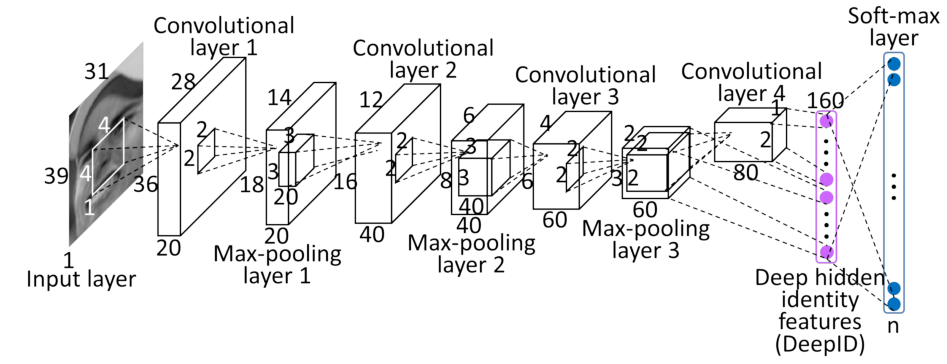
\includegraphics[width=\textwidth]{figures/deepid_convnet}
	\caption{Structure of the \gls{cnn} used in \gls{deepid} \citep{deepID2014}}
	\label{fig:deepid_convnet}
\end{figure}

\subsection{DeepID2}
\gls{deepid2} is an expansion upon \gls{deepid} and is a deep \glsentrylong{cnn} used for face identification and verification. This is done by using feature extraction.

Just like \gls{deepid}, \gls{deepid2} uses four convolutional layers but only the first three uses max-pooling. It uses 400 face patches instead of 60 \citep{deepID2014,sun2014} and detects 21 landmarks of the face.

The \gls{deepid2} layer is after the four convolutional layers. This layer is learned under two supervisory signals. The first is identification classifying the images into identities. The second is face verification which manipulates the \gls{deepid2} data to be similar to a matching identity should this be the same. \autoref{fig:deepid2_convnet} shows the structure af the \gls{deepid2} network.

\gls{deepid2} also uses the \gls{lfw} database and achieves a $99.15\%$ accuracy.

\begin{figure}[h]
	\centering
	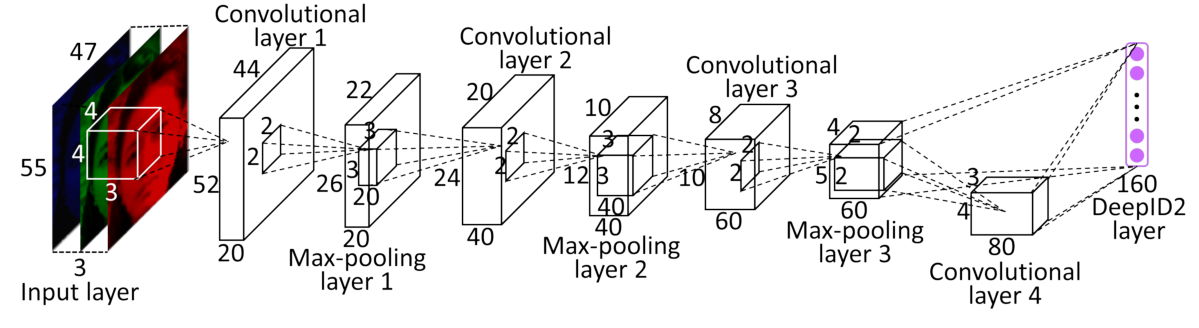
\includegraphics[width=\textwidth]{figures/deepid2_convnet}
	\caption{Structure of the \gls{cnn} used in \gls{deepid2} \citep{sun2014}}
	\label{fig:deepid2_convnet}
\end{figure}

\subsection{DeepID3}
DeepID3 is a further expansion of both \gls{deepid} and \gls{deepid2} but is also drawing on some from elements from VGG net and GoogleNet \citep{sun2015}. The qualities from these two networks is the use of stacked convolution and inception layers. DeepID3 is in general a deeper network than \gls{deepid2} and its expansion \gls{deepid2}+. However, DeepID3 resembles \gls{deepid2} in the use of adding supervisory signals to early layers.

\cite{sun2015} proposes two different networks with DeepID3. One is using eight convolutional layers with max pooling after every other convolutional layer. The second network has four convolutional layers with max pooling after every other, following are five inception layers. These two networks are shown in \autoref{fig:deepid3_net}.

DeepID3 is also tested on the \gls{lfw} dataset with an accuracy of $99.52\%$, which is an increase in accuracy compared to \gls{deepid2} but as stated in \cite{sun2015} it is not an improvement of \gls{deepid2}+.

\begin{figure}[h]
	\centering
	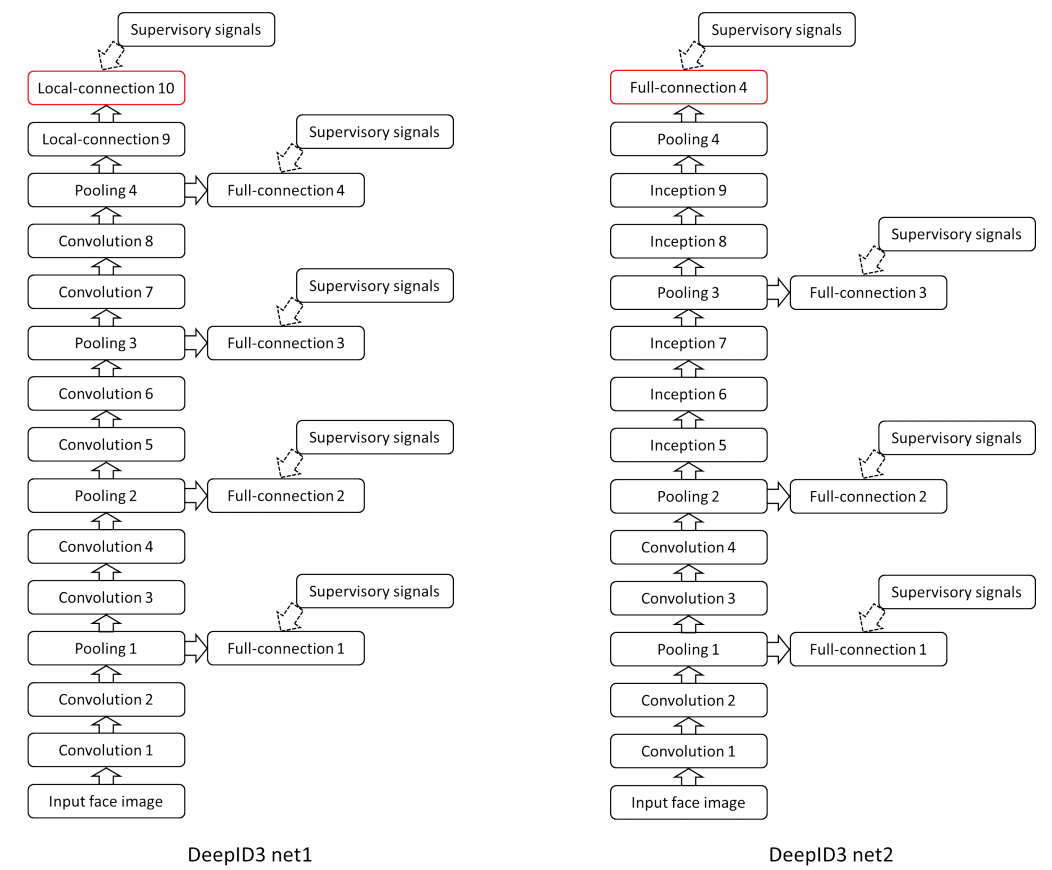
\includegraphics[width=\textwidth]{figures/deepid3_net}
	\caption{Structure of the \gls{cnn}s used in DeepID3 \citep{sun2015}}
	\label{fig:deepid3_net}
\end{figure}

\hl{The other biometric trait that is considered} in the work in this project is the iris. \autoref{sec:Iris_Recognition_Research} summarises the state of the art methods as well as the commonly used methods for iris processing and classification.  
\section{Iris Recognition}
\label{sec:Iris_Recognition_Research}
Modern iris recognition was first introduced in an article by \cite{Daugman1993} discussing the security of using iris for recognition. Here an outline of how to do recognition was laid out and even though the field has been extensively \todo{extensively what?} since, the general methodology is more or less the same as Daugman proposed. A modern system is typically composed of image acquisition, segmentation and normalisation, feature extraction and matching. 

\subsection{Images}
The images acquired are often taken in the \gls{nir} spectrum, which is ranging between 700 nm and 900 nm in wavelength. In this band, the melanin in the iris, which is the substance that gives the iris its colour e.g. brown or blue, is typically less prominent making the unique structure in the iris very distinct. To acquire usable \gls{nir} images, the user has to be in the millimetre range of the \gls{nir} camera. In the visible light, the melanin is much more prominent and thus makes is harder to detect the structure. The band of visible light has many names in the literature, namely Visible Spectrum (VIS), Visible Wavelength (VW), and \gls{vl}. \gls{vl} will be used in this report. While \gls{nir} is beneficial in some cases, other useful features can be observed in the \gls{vl} that cannot be seen with \gls{nir}. These can include the moles, freckles and conjunctival vasculature, which can help in making more accurate recognition systems. To make iris recognitions systems comparable with each other some publicly available databases are often used. \cite{Rifaee2017}  give an outline of the some of the free databases that are used. A comprehensive table summarising the visual properties, statistics and type of subject used in various database are tabulated in \autoref{fig:Iris_database_1} and \autoref{fig:Iris_database_2}. Most of the databases available are \gls{nir} images with CASIA being one of the most used database. For \gls{vl} images, UBIRIS in the most commonly used. These contain more "real world" data as the images contain more noise in the form of eyelids obstruction, eyelash obstruction, glare, motion blur, out-of-focus or poor focused iris, partial iris and specular reflection \citep{Rattani2017}. The database has also been used in Noisy Iris Challenge Evaluation (NICE) I. The increasing usage of mobile devices also proposes an opportunity to integrate iris recognition as a biometric for verifying the identity of the user. For this purpose a competition, Mobile Iris CHallenge Evaluation (MICHE), is made to compare the state of the art mobile iris. They provide a the MICHE database that can be used, which they claim is a better database than UBRIS for mobile systems. The database contains noisy iris images taken with a Galaxy Samsung IV, iPhone 5, and Galaxy Tablet II. The noise includes noise from both artificial and natural light sources during acquisition, motion blur, occlusion due to eyelids, glasses, eyelashes, hair, or shadows, which can naturally occur when a user is trying to unlock a phone using their iris. 

\begin{figure}[H]
\centering
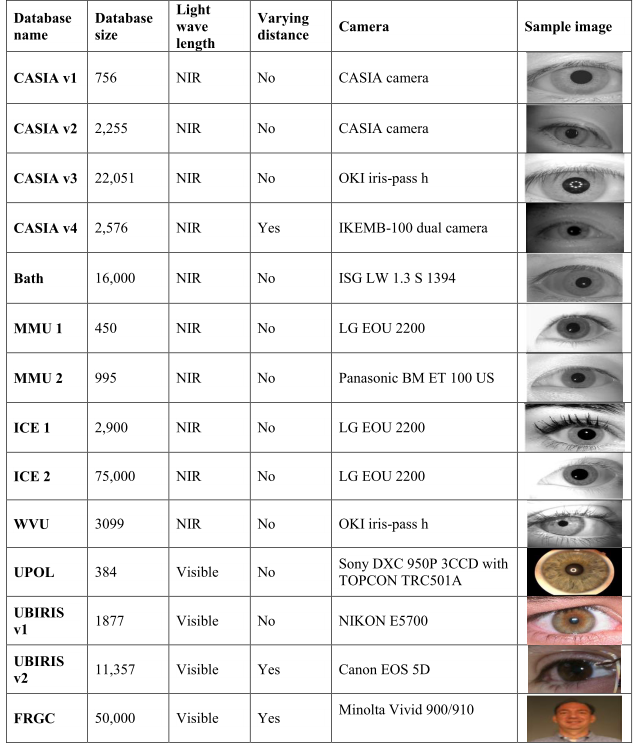
\includegraphics[width=\textwidth]{figures/Iris_Database_tabel_1.png} 
\caption{A table depicting the contents of free iris image databases  \citep{Rifaee2017}.}
\label{fig:Iris_database_1}
\end{figure}

\begin{figure}[H]
\centering
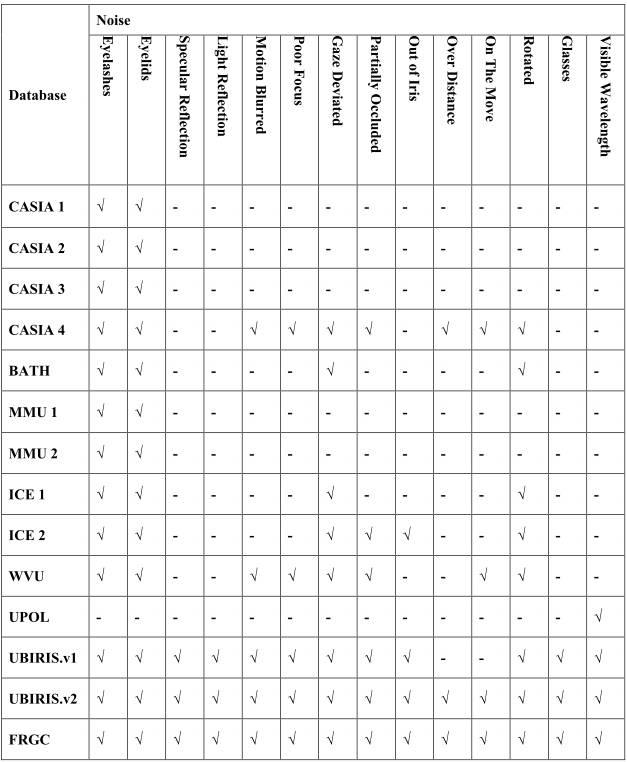
\includegraphics[width=\textwidth]{figures/Iris_Database_tabel_2.png} 
\caption{A table depicting the noise present in the databases  \citep{Rifaee2017}.}
\label{fig:Iris_database_2}
\end{figure}


\subsection{Segmentation}
Segmentation of an iris in iris recognition systems tries to detect the iris and find the pupillary boundary and the limbus boundary as well the eyelids and eyelashes that can cause noise on the image. The boundaries along with other parts of the iris can be seen in \autoref{fig:iris_naming}. The approach used for segmentation depends among other things on the wavelength of the image; \gls{nir} or \gls{vl}. They both have some common challenges to them. Often the eyelids can cover a small part of the iris, causing the limbus boundary of the iris to not be circular or elliptical. Eyelashes can also cause a similar disturbance as they also can cover parts of the iris. Poor lighting can also make it extremely difficult to detect the boundaries. Specular reflections in the iris can also cause difficulties as they can lie on the iris boundary or close to. Most systems also require a great deal of user cooperation as an off angle iris, motion blur, or glasses or contact lenses can make it even more difficult to detect the boundaries. This can especially be the case for iris recognition in a phone as it cannot be expected of the user knows how to acquire a good iris image. 

\begin{figure}[H]
\centering
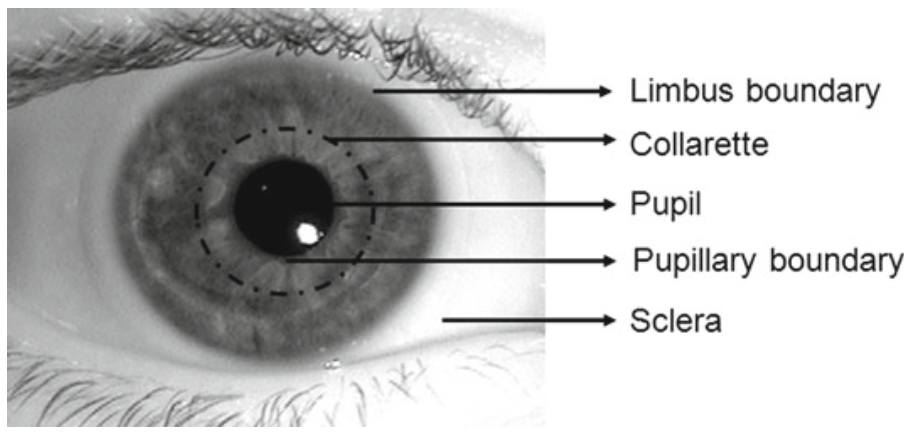
\includegraphics[width=\textwidth]{figures/iris_naming.png} 
\caption{A close up \gls{nir} image of an iris depicting the different parts of the iris along with their names \citep{Bowyer2016b}}
\label{fig:iris_naming}
\end{figure}

Two commonly observed approaches for segmentation in \gls{nir} band images are Daugman's approach \citep{Daugman1993} , \citep{Saha2017}, \citep{Rattani2017}, \citep{Khan2017a}, and Hough Transform \citep{Luhadiya2017}, \citep{Uka2017}. Daugman's approach consists of using a Gaussian filter on the image to attenuate the effect of noise and eliminate undesired weak edges like the boundaries within the iris while keeping the strong edges like iris boundaries and eyelid boundaries. An integro-differential operator is then used as a circular edge detector. It is then used iteratively to find the pupillary boundary and the limbus boundary. Hough Transform on the other hand is a histogram based model fitting approach. An edge map of the input map is generated using a gradient-based edge detector. Then a voting procedure is applied on the thresholded edge map to determine the parameters for a contour that best fits a circle. This operation gives an approximate edge map of the iris boundary. Lastly, the segmented iris is often normalised using Daugman's rubber sheet model that maps every point in the segmented region from cartesian to polar coordinates. An open source MATLAB implementation based on updated version of the Daugman approach is a commonly used tool\todo{Remember to add a proper citation}. There exist other methods for different circumstances, but these are two most commonly used. They can also be used on \gls{vl} images if the image is converted from RGB to grey scale images \citep{Bowyer2016b} \todo{How to properly cite a book where each chapter is written by different people?}. 

\subsection{Feature extraction and classification}
There are multiple ways that the features can be extracted from the segmented iris. The most commonly used in the literature is a 2D Gabor filter which is a linear filter used for edge detection \citep{Daugman1993}. The Hamming distance is then used as way to classify the iris. The Hamming distance is a measurement of how many bit flips a piece of data need to have to match another piece of data. The bits of the extracted features are then measured against the whole database and the pair with the lowest score is a match. This is called "1-to-N search". As the database gets larger and larger the computation time also grows as it will have to search through the whole database. That's why \cite{Kuehlkamp2016} have suggested using a "1-to-first search" instead to improve the speed of the search. Here a threshold is chosen and as soon as a match has been found below the threshold it will stop the search. Other approaches to the categorisation have been proposed using machine learning. \cite{Khan2017} proposed using \gls{svm}, \gls{knn} and \gls{lda} with respective test accuracies of 97\%, 95.1\%, 94.28\%. In comparisons the  commercial systems ranged from 94.57\% to  99.67\% with VeriEye having the lowest and IriCore having the highest accuracy. 

\subsection{Deep Learning}
According to \cite{Zhao2017a} research in neural networks within iris recognition is still very new and not much has been done. Some of the work that has been done have used \gls{cnn} and a \gls{dbn}. \cite{Al-Waisy2017} used a common \gls{cnn} to extract features and classify a segmented and normalised iris image. The segmentation was done using Circular Hough Transform (CHT) normalisation was done using Daugman's rubber sheet method. They named the network IrisConvNet and the architecture was inspired by the Spoofnet \todo{maybe add a source or explanation if needed?}  as it can be seen in \autoref{fig:Al_Waisy2017_CNN_model}. This was the general architecture and they tried different numbers of maps and layers to find the best architecture. In general a 3x3 input kernal was used on a 64x64 or 128x128 pixel input image to create feature maps followed by 2x2 max pooling, 5x5 convolution, 2x2 max pooling 5x5 convolution, 2x2 max pooling, 5x5 convolution and finally a two fully connected layers to to a softmax regression classifier layer. A ReLU activation function is applied on the top of the convolutional and fully connected layers because it results in several times faster training without sacrificing accuracy. The AdaGrad algorithm was used for training the network. Three databases were used; SDUMLA-HMT, CASIA-Iris-V3 and IIT Dehli (IITD). IrisConvNet scored an accuracy of 99.82\% at categorising CASIA-Iris-V3 in 0.65 s. architecture 

\begin{figure}[H]
\centering
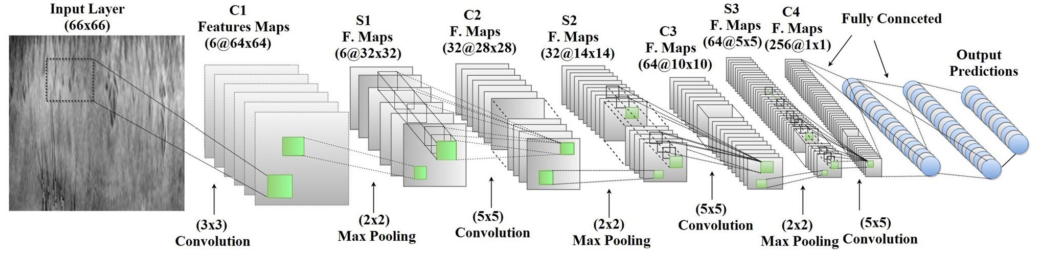
\includegraphics[width=\textwidth]{figures/Al_Waisy2017_CNN_model.png} 
\caption{Example of a \gls{cnn} architecture  from \cite{Al-Waisy2017}.}
\label{fig:Al_Waisy2017_CNN_model}
\end{figure}


\cite{Zhao2017a} claim that the problem with traditional networks are that they are database specific and not very generalisable. They created a \gls{fcn} using a loss function they created specifically for iris networks called Extended Triplet Loss (ETL). They claim this network is more generalisable than the previous networks and it shows superior results compared with IrisCode\todo{IrisCode? what is this?} which is Daugman's segmentation and normalisation approach. A \gls{fcn} differs from a \gls{cnn} in that there are no fully connected layers, only convolutional layers, max pooling etc. They proposed an architecture called UniNet that can be seen in \autoref{fig:Zhao2017_CNN_model}. It consists of two \gls{fcn}s; FeatNet and MaskNet. The network takes an iris that has been segmented and normalised using a recent approach \citep{Zhao2015a}. The segmented iris has a resolution of 64x512 pixels. The image is then fed through FeatNet and MaskNet. FeatNet extracts the iris features while MaskNet masks the non-iris part of the image. e.g an eyelid that occludes.  Three of these UniNet networks are then trained in parallel in Triplet-based network architecture that uses the ETL loss function. They used four databases to train and the networks; ND-IRIS-0405, CASIA V4, IITD and WVU Non-ideal Iris Database. It was then compared with a \gls{cnn} network based on VGG-16 that used softmax, \gls{cnn} with triplet, FeatNet only and DeepIrisNet which is a \gls{cnn} that is proposed directly for iris recognition. The results can be seen in \autoref{fig:Zhao2017_CNN_results} where UniNet outperforms the other nets and FeatNet is the by far worst performing network, which suggests that MaskNet is needed for the network to perform well. 

\begin{figure}[H]
\centering
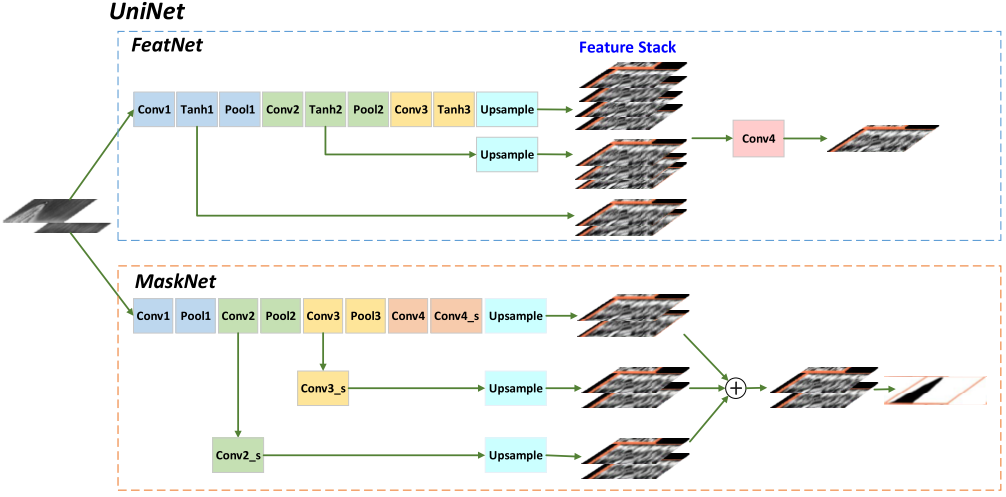
\includegraphics[width=\textwidth]{figures/Zhao2017_CNN_model.png} 
\caption{Example of a \gls{cnn} architecture  from \cite{Zhao2017}.}
\label{fig:Zhao2017_CNN_model}
\end{figure}

\begin{figure}[H]
\centering
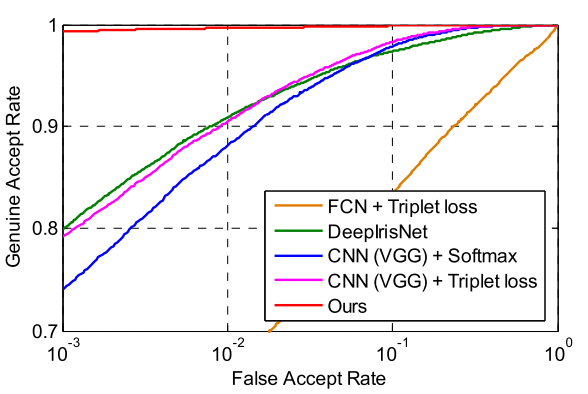
\includegraphics[width=\textwidth]{figures/Zhao2017_CNN_results} 
\caption{Results from the different networks tested on the ND-IRIS-0405 database  \cite{Zhao2017}. "Ours" is UniNet and FCN + Tripletloss is FeatNet}
\label{fig:Zhao2017_CNN_results}
\end{figure}


Another promising approach by \cite{Bazrafkan2017} targets iris segmentation in low-quality consumer images obtained from smartphones is using \gls{spdnn} for generating iris maps from low quality iris images.  In \gls{spdnn} several deep networks are merged into a single model. This way it is possible to include different networks designs and combine their strengths. They combined four \gls{fcn}s of different architectures that used a variaty of kernel sizes and layers. An example of one of the \gls{fcn}s has 12 convolutional layers  in this order; 3x3,5x5,7x7,9x9,11x11,13x13,15x15,13x13,11x11,9x9,7x7,5x5 and an output layer that is 3x3.It was trained by using the databases Bath800, CASIA Thousand, UBRIS and MobBio. They contained both \gls{nir} and \gls{vl}\todo{consider whether it makes sense to call it VL images rather than RGB images} images. Extensive noise was also added to the training images in the form of blur and lower contrast to generate degraded versions of the high quality images and utilise the databases better by creating more samples. Using the UBRIS database as a comparison with other state of the art segmentation techniques it achieved the highest accuracy with 99.30\%. The technique with the lowest accuracy, of the ones it was compared to, had an accuracy of 98.10\%.   









%\cite{Rifaee2017} gives an outline of commercially free databases often used in research.\autoref{fig:Iris_database_1} and \autoref{fig:Iris_database_2} show the different contents of the databases. Most of the databases are \gls{nir} images with CASIA being one most used databases in the literature.  For images in the visible light UBRIS is often used . These contain more "real world" data as the images contain more noise in the form of eyelids obstruction, eyelash obstruction, glare, motion blur, out-of-focus or poor focused iris, partial iris and spec- ular reflection \citep{Rattani2017}. The database has also been used in Noisy Iris Challenge Evaluation (NICE) I. For iris recognition system on mobile platforms the Mobile Iris CHallenge Evaluation (MICHE) database can be used.  The database contains noisy images taken withe Galaxy Samsung IV, Iphone5 and Galaxy Tablet II. The noise includes noise from both artificial and natural light sources during acquisition, motion blur, occlusion due to eyelids/glasses/eyelashes/hair/shadows which can naturally occur when a user is trying to unlock a phone using their iris. 


%. It was also the foundation for IrisCode which is a commercially developed iris recognition algorithm by John Daugman. In 2016 a handbook for iris recognition by \cite{Bowyer2016b} was published giving an outline of the whole process of iris recognition. In general Near Infra-Red (NIR) images of an iris are used but other type of images can also be used.  \cite{Khan2017a} show how to use Daugmans methodology on iris images taken with a smartphone in visible light. They use Daugmans Integro-differential operator to localise the bounds of the iris. Then they suppress the eyelids the eyelids which often cover parts of the iris by using an approach inspired by Masek. Afterwards the image is normalised by using the homogeneous rubber sheet model by Daugman. Then eyelashes are removed from the image and feature extraction is done by using 2D Gabor Waveletts. This approach to extract features in one way or another can be seen in multiple state of the art iris recognition systems and research papers e.g \citep{Luhadiya2017a,Uka2017a,Kuehlkamp2016a}, \cite{Kuehlkamp2016a}. After the features have been extracted they are compared/categorised. Traditionally a "1-to-N search" has been done. Here the Hamming distance of features of the scanned iris are compared to the whole database and it is classified with the iris that has the least distance. \cite{Kuehlkamp2016a} have suggested using a "1-to-first search" instead to improve the speed of the search. Here a threshold is chosen and as soon as a match has been found below the threshold it will stop the search. Other approaches to the categorisation have been proposed using machine learning. \cite{Khan2017a} proposed using Support Vector Machines (SVM), K-Nearest-Neighbours(KNN) and Linear Discriminant Analysis (LDA) with respective test accuracies of 97\%, 95.1\%, 94.28\%. \cite{Zhao2017b} proposed using deep learning to classify. They claim that research in neural networks with iris recognition is still very new and not much has been done. But some of the work that has been done have used Convolutional Neural Networks (CNN) and a Deep Belief Network (DBN). They claim that the problem with traditional networks are that they are very database specific on not very generalisable. \cite{Zhao2017b} created a Fully Convolutional Network (FCN) using a loss function they created specifically for iris networks called Extended Triplet Loss (ETL). They claim this network is more generalisable than the previous networks. 







\section{Information fusion and face-iris databases}

A system that strives to utilise information from two or more different biometric traits in order to obtain one result is a called a multi-modal which is a kind multi-biometric system. Besides the multi-modal approach there are several other approaches, which results in information from two or more sources, therefore, methods for fusion of information from different sources into one system for recognition purposes a widely investigated area.  The fusion can happen on different levels. It can happen on one of five levels: signal level, feature level, score level, rank level, or on the decision level. In general score-level and feature-level are the most popular fusing techniques \citep{Bowyer2016b}. For each of the fusing techniques there are several approaches to how to do the fusing. For the lowest level, signal level, the fusing might be merging data from different sources to construct a more detailed dataset or signal. On the feature level the fusing might happen through merging of extracted features from different sources into one feature vector \citep{Ross2003}. On the score level it can be determining the best sample to use for the processing based on which is has the highest score and is the best match to the gallery samples. Rank level can be similar to the scores but dependent on match rankings, on decision level it can be applying Multiple Classifier Systems, e.g. one for each modality\citep{Fierrez2018b}. 
Even though recognition based on biometric traits is widely investigated, and research shows that multimodal systems perform better than the uni-modal systems based on the same data, the research in this area is limited and incomplete. Because of the limited access to multimodal datasets, such datasets are often synthetically constructed based on randomly combined iris and face datasets. Only a limited amount of studies on actual utilise a multimodal dataset obtained like that. The named multimodal datasets encountered in literature are the dataset $IV^2$ and the datasets provided for the The Multiple Biometric Grand Challenge\citep{Bowyer2016b,Petrovska-Delacretaz2008a}. The latter is available on request and also serves as a common test set in order to compare performance.  

Based on the knowledge gained from the research done, a set of requirements regarding the development of a solution are constructed. This is done to measure the quality of the solution.
%\graphicspath{{figures/analysis/}}
\chapter{Analysis}\label{ch:analysis}
\section{Face Recognition}
The first computer based face recognition was made in 1973. This was based on a feature approach, meaning the program identifies basic face features such as mouth, eye, and nose placement. 
From here three different types of approaches emerged, namely a holistic, feature extraction and a hybrid approach. 

The holistic approach encodes the entirety of a face and then identifies using template-matching, the feature extraction approach extracts a defined amount of features from the face, whereas the hybrid method uses both template-matching and feature extraction \citep{Wechsler2007}.
In 1990, \gls{pca} was introduced for holistic face recognition. The \gls{pca} approach makes use of eigenfaces, each eigenface represents a principal component in which a face is encoded. But as \cite{Wechsler2007} claims, \gls{lda} is a more effective suitable approach for face identification and authentication. Another holistic approach is using \gls{svm} for face recognition \citep{Wechsler2007}.

The feature approach gave way for what is now known as recognition-by-parts, which uses the features and a global structure to link these features. A structure for linking 2D features is the \gls{hmm}. \gls{pca} is also used in this approach, but is used to model shape or texture of the face.

In the late 2000s deep learning was introduced with representation-learning methods with multiple levels of representation. By feeding raw data and finding and emphasising on the important aspects of the data and suppressing the unimportant ones, higher level classification is possible \citep{LeCun2015}. This is done with several \textit{hidden layers}. The more layers there are, the deeper a network is said to be. 

In the following some of the state of the art deep learning networks for face recognition are presented.

\subsection{DeepID}
\gls{deepid} is a \gls{cnn} which aims to use feature extraction for face identification and verification. It detects five facial landmarks; the two eye centres, the nose tip, and the two mouth corners. The network is made of four convolutional layers with max-pooling, which are used to extract features hierarchically. These are followed by the fully-connected \gls{deepid} layer and a softmax output layer to indicate identity classes. The feature extraction and face recognition is done in two steps, where the first step, feature extraction, is learned with the target of face identification \citep{deepID2014}.

In the \gls{cnn}s the neuron number of the last hidden layer in the network is much smaller than that of the output layer. This is done, to better classify faces \citep{deepID2014}. The network extracts low-level features in the bottom layers, where feature numbers decreases for each layer. In opposition, the high-level features are formed in the top layers. An overview of the network structure is shown in \autoref{fig:deepid_convnet}.

The network is tested using the \gls{lfw} database. This database is images of faces from different angles and scenarios consisting of 13.233 images from 5749 subjects. However, only 1680 of the subjects are sampled more than twice \citep{lfw2007}. It achieves $97.45\%$ accuracy on this dataset, requiring weakly aligned faces \citep{deepID2014}.

\begin{figure}[h]
	\centering
	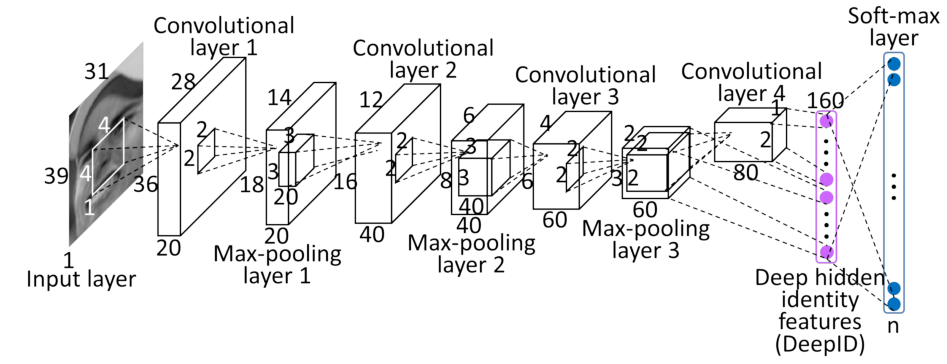
\includegraphics[width=\textwidth]{figures/deepid_convnet}
	\caption{Structure of the \gls{cnn} used in \gls{deepid} \citep{deepID2014}}
	\label{fig:deepid_convnet}
\end{figure}

\subsection{DeepID2}
\gls{deepid2} is an expansion upon \gls{deepid} and is a deep \glsentrylong{cnn} used for face identification and verification. This is done by using feature extraction.

Just like \gls{deepid}, \gls{deepid2} uses four convolutional layers but only the first three uses max-pooling. It uses 400 face patches instead of 60 \citep{deepID2014,sun2014} and detects 21 landmarks of the face.

The \gls{deepid2} layer is after the four convolutional layers. This layer is learned under two supervisory signals. The first is identification classifying the images into identities. The second is face verification which manipulates the \gls{deepid2} data to be similar to a matching identity should this be the same. \autoref{fig:deepid2_convnet} shows the structure af the \gls{deepid2} network.

\gls{deepid2} also uses the \gls{lfw} database and achieves a $99.15\%$ accuracy.

\begin{figure}[h]
	\centering
	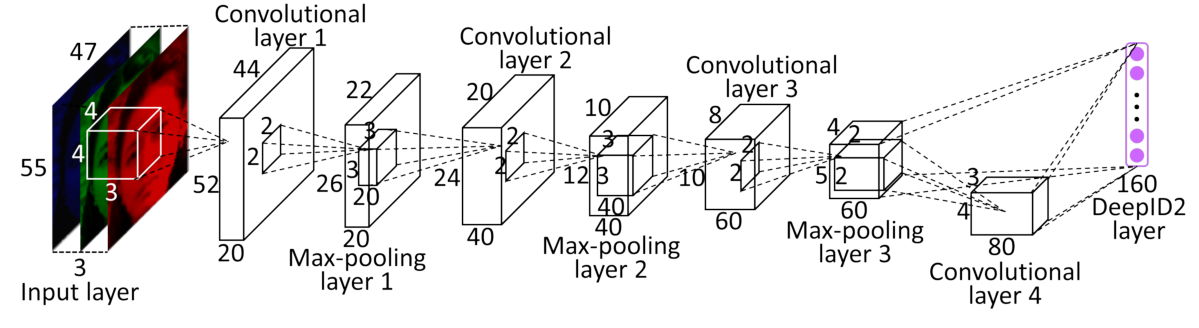
\includegraphics[width=\textwidth]{figures/deepid2_convnet}
	\caption{Structure of the \gls{cnn} used in \gls{deepid2} \citep{sun2014}}
	\label{fig:deepid2_convnet}
\end{figure}

\subsection{DeepID3}
DeepID3 is a further expansion of both \gls{deepid} and \gls{deepid2} but is also drawing on some from elements from VGG net and GoogleNet \citep{sun2015}. The qualities from these two networks is the use of stacked convolution and inception layers. DeepID3 is in general a deeper network than \gls{deepid2} and its expansion \gls{deepid2}+. However, DeepID3 resembles \gls{deepid2} in the use of adding supervisory signals to early layers.

\cite{sun2015} proposes two different networks with DeepID3. One is using eight convolutional layers with max pooling after every other convolutional layer. The second network has four convolutional layers with max pooling after every other, following are five inception layers. These two networks are shown in \autoref{fig:deepid3_net}.

DeepID3 is also tested on the \gls{lfw} dataset with an accuracy of $99.52\%$, which is an increase in accuracy compared to \gls{deepid2} but as stated in \cite{sun2015} it is not an improvement of \gls{deepid2}+.

\begin{figure}[h]
	\centering
	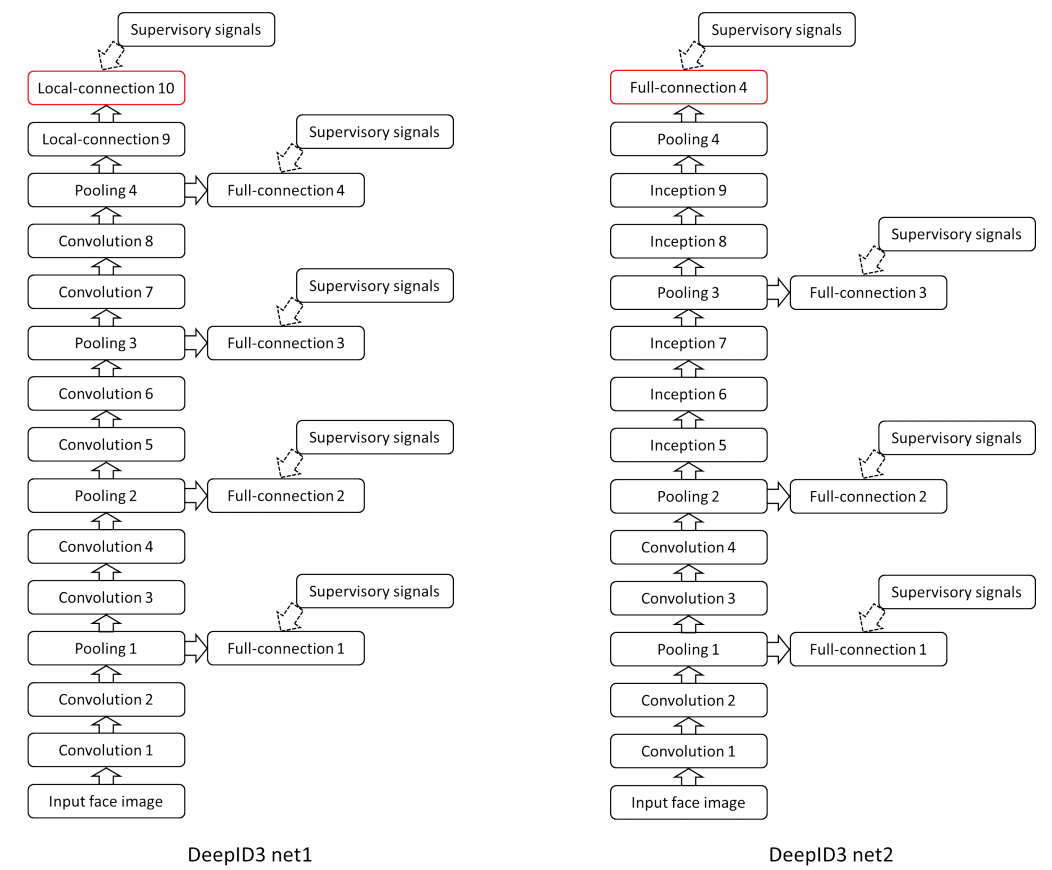
\includegraphics[width=\textwidth]{figures/deepid3_net}
	\caption{Structure of the \gls{cnn}s used in DeepID3 \citep{sun2015}}
	\label{fig:deepid3_net}
\end{figure}

\hl{The other biometric trait that is considered} in the work in this project is the iris. \autoref{sec:Iris_Recognition_Research} summarises the state of the art methods as well as the commonly used methods for iris processing and classification.  
\section{Iris Recognition}
\section{Face and Iris Fusion}

%\chapter{Problem Statement}

%\chapter{Requirements}\label{ch:req}\glsresetall
To be able to measure the quality of the identification method made, a set of requirements are presented. These are produced on the background of knowledge presented in \autoref{cha:Research}.

The context of the work carried out is identity verification on smart phones. Therefore, there are certain requirements to the system. Although some smartphones nowadays are equipped with \gls{nir} cameras not all are. Therefore, it would be beneficial if successful identity verification proved possible when using the normal \gls{vl} front camera, which most smartphones are equipped with, as this requires less sensors and thus is cheaper for the smart phone manufacturers. From these considerations two requirements for the system arises. The input images used for the identification has to be \gls{vl} images, and furthermore, the images have to have a resolution, which is low enough to represent the images that would be captured with a smart phone front camera.

Furthermore, the system has to identify using one of the biometric modalities face, or iris, or both, since those are the most reliable non-invasive biometric traits, which can be obtained by a smart phone and especially with a \gls{vl} camera. 

The designed solutions must have an accuracy comparable to the ones of state of the art solutions and commercial systems presented in \autoref{cha:Research}. The accuracies presented are generally at $99\%$ or above, which means the solution implemented in this project must have an accuracy equal to or above this accuracy as well. 

The solution for identification based on fusion of the two modalities has to have an accuracy higher than the accuracies of the system based on the individual modalities for it to be accepted. If the accuracy is the same, there is no gain in the increased computational complexity of a multimodal system and as a result the system will be forsaken.\todo[inline]{Add delimitation from computational limitations and requirements for the computational time} 
%As the project seeks to make a better verification for security measures, the fused networks should perform better than that of the non-fused.


%\graphicspath{{figures/design/}}
\chapter{Design}\label{ch:design}


%\graphicspath{{figures/implementation/}}
\chapter{Implementation}\label{ch:implementation}



\section{Basic Methods}
\label{BasicM}
In order to get some basic understanding of the methods commonly used for iris classification the work presented in an article is implemented. The work implemented is the work of \cite{Khan2017a} described in \textit{Iris Recognition using Machine Learning from Smartphones Captured Images in Visible Light}. In the work the database Warsaw-BioBase containing \gls{vl} images of the iris obtained by smartphones are processed and used to train different classifiers. The images of this database comply with the requirements set for this work mentioned in \autoref{ch:req}.\todo[author=Niclas]{Angiv database størrelse og evt. billedeopløsning.} The processing consists of a sequence of steps. The steps included are

\begin{itemize}
\item Iris Location
\item Eyelid Suppression
\item Iris Normalisation
\item Noise Removal
\item Histogram Equalisation 
\item Feature Extraction
\item Training and Classification
\end{itemize}
\autoref{fig:ExWars} shows an example of an image from the database. Before the first step some simple preprocessing is done. The red channel is preserved and the other two colour channels are neglected. This is done because this simulates the use of \gls{nir} light. The result is a greyscale image based on the red channel. In the following sections the implementation of each of the steps is elaborated. 

\begin{figure}[h]
\centering
\begin{subfigure}{.47\textwidth}
\centering
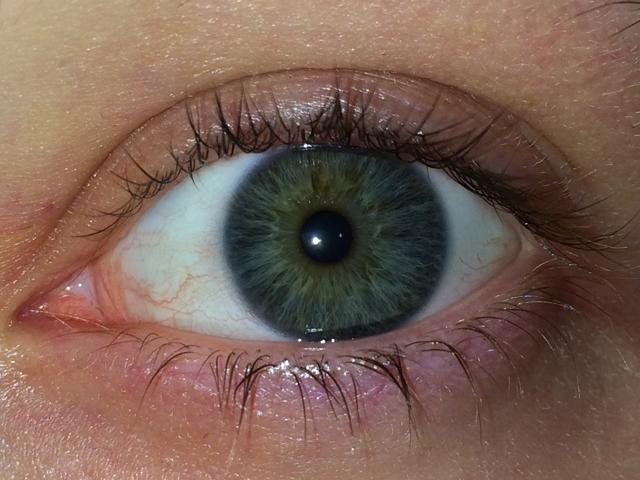
\includegraphics[width=0.90\textwidth]{IMG_1838.jpg}
\caption{Example of visible light image of an iris from the used database.}
\label{fig:ExWars}
\end{subfigure}
~
\begin{subfigure}{.47\textwidth}
\centering
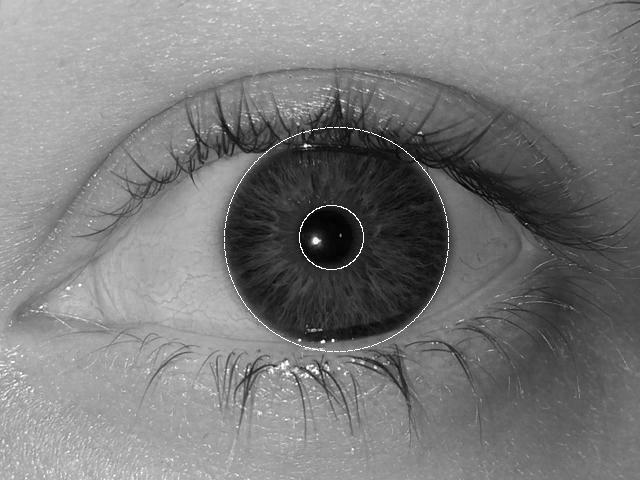
\includegraphics[width=0.90\textwidth]{0002left_13-marked.jpg}
\caption{The eye marked with the identified edges of the iris.}
\label{fig:MarkedI}
\end{subfigure}

\begin{subfigure}{.47\textwidth}
\centering
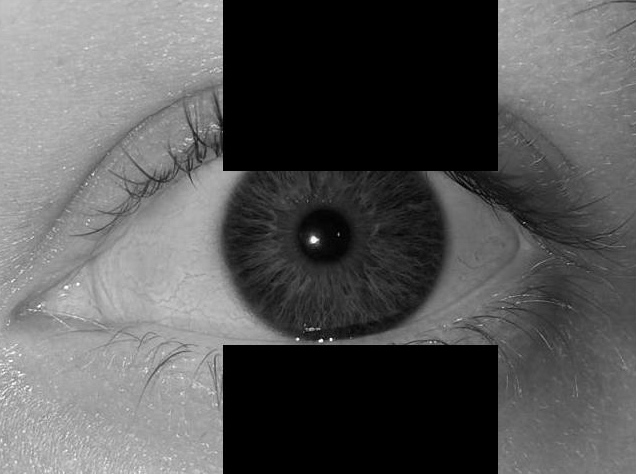
\includegraphics[width=0.9\textwidth]{Eyelid_002_l_13_2.jpg}
\caption{The eye with the eyelid suppression applied.}
\label{fig:IrisSup}
\end{subfigure}
\caption{The original image before and after different steps of processing.}
\end{figure}



\subsection{Iris Segmentation}
The first step of processing is locating the iris. For this purpose Daugman's Integro-differential operator is used. The operator identifies the circular contour, which has the greatest change in intensity by varying the three parameters defining the circle $(r,x_0,y_0)$, radius and centre coordinates. The operator is defined by the formula in \autoref{eq:integro_diff}.

\begin{equation}\label{eq:integro_diff}
	\max(r,x_{0},y_{0}){\left|G_{\sigma}{(r)*}{\partial\over \partial_{r}}{\oint_{r,x_{0},y_{0}}}{{I(x,y)\over 2\pi r}dS}\right|}
\end{equation}
Where $I(x,y)$ is the intensity or grey level of the image at the coordinates (x,y), $S$ is the circle, and $G_{\sigma}{(r)}$ is a Gaussian smoothing function.
The method is also used to find the edge between the pupil and the iris. The two identified edges are marked on the input image. \autoref{fig:MarkedI} shows an example of the identified edges of the iris. 

\subsection{Eyelid Suppression}
The annulus, which lies between the two borders identified during the iris extraction might not only contain the iris. The subject might in some cases not open the eyelids fully or the angle of the camera might be such that parts of the iris is covered by the eyelids. Therefore, an algorithm which eliminates the eyelids is used. 
The algorithm is applied on the image cutout of the original image, which is bound by the boundary box of the identified iris. The small image is divided into an upper and a lower part, which are searched for the upper and the lower eyelid respectively. The search is done by using a method with some similarities to Daugman's Integro-differential operator shown in \autoref{eq:integro_diff}, however it applies radon transform. Through the output of the radon transform the lines marking the two eyelids are found and the pixels above or below the two lines respectively are eliminated. The resulting image is shown in \autoref{fig:IrisSup}.

\subsection{Iris Normalisation}
\label{sec:irisnorm}
For the normalisation, Daugman's Rubber Sheet Model is used. The purpose is to get a rectangular image of the iris, which corresponds to taking the annulus covered by the iris region, cutting it open and unfolding or stretching it to a rectangular shape. 

\begin{figure}[h]
\centering
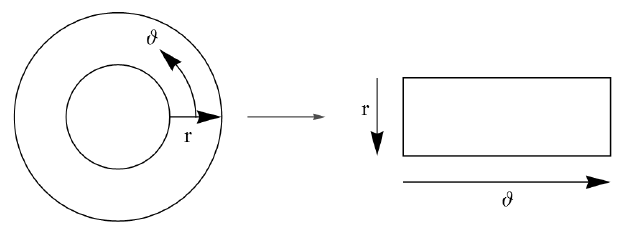
\includegraphics[width=0.8\textwidth]{Daugmans-Rubber-Sheet-Model.png}
\caption{Daugman's Rubber Sheet Model. \citep{Misztal2012}}
\label{fig:DaugSheet}
\end{figure}

The model does this by mapping the iris from the original image to a rectangular image. The mapping is done based on polar coordinates, radius, and angle, $(r,\vartheta)$, where $r\in[0,1]$ and $\vartheta\in[0,2\pi]$. In the rectangular image angle $\vartheta$ is on the x-axis and the radius $r$ is on the y-axis of the image. \autoref{fig:DaugSheet} shows the mapping of the method. This was implemented using a function in the library crated by Libor Masek \citep{LiborMasek2003}. The resolution of the resulting image is dependent on arguments. In this work the dimensions are set to be $64\times512$. The image of the normalised iris is shown in \autoref{fig:SimPolar}. 

\begin{figure}[h]
\centering
\includegraphics[width=\textwidth]{002polar.jpg}
\caption{The normalised image of the iris before applying functions.}
\label{fig:SimPolar}
\end{figure}

\subsection{Noise Removal}
Though the article uses several well known methods, which are commonly used in processing of images of irises, the descriptions of the methods are quite inadequate. The description of the noise removal is an example hereof. After obtaining the normalised iris, the next step applied is noise removal. The purpose of the noise remover function is to remove noise occurring in the form of eyelashes covering parts of the iris. Usually the pixels showing the lashes will be among the darkest pixels. Since every image of an iris is different and how dark the iris is also varies, a threshold has to be identified adaptively. The article does not describe in depth how this is implemented, it simply states that some histogram analysis is done in order to obtain the lowest pixel values. \autoref{fig:histBif} shows the histogram of the normalised image before any noise removal. 

\begin{figure}[H]
	\centering
	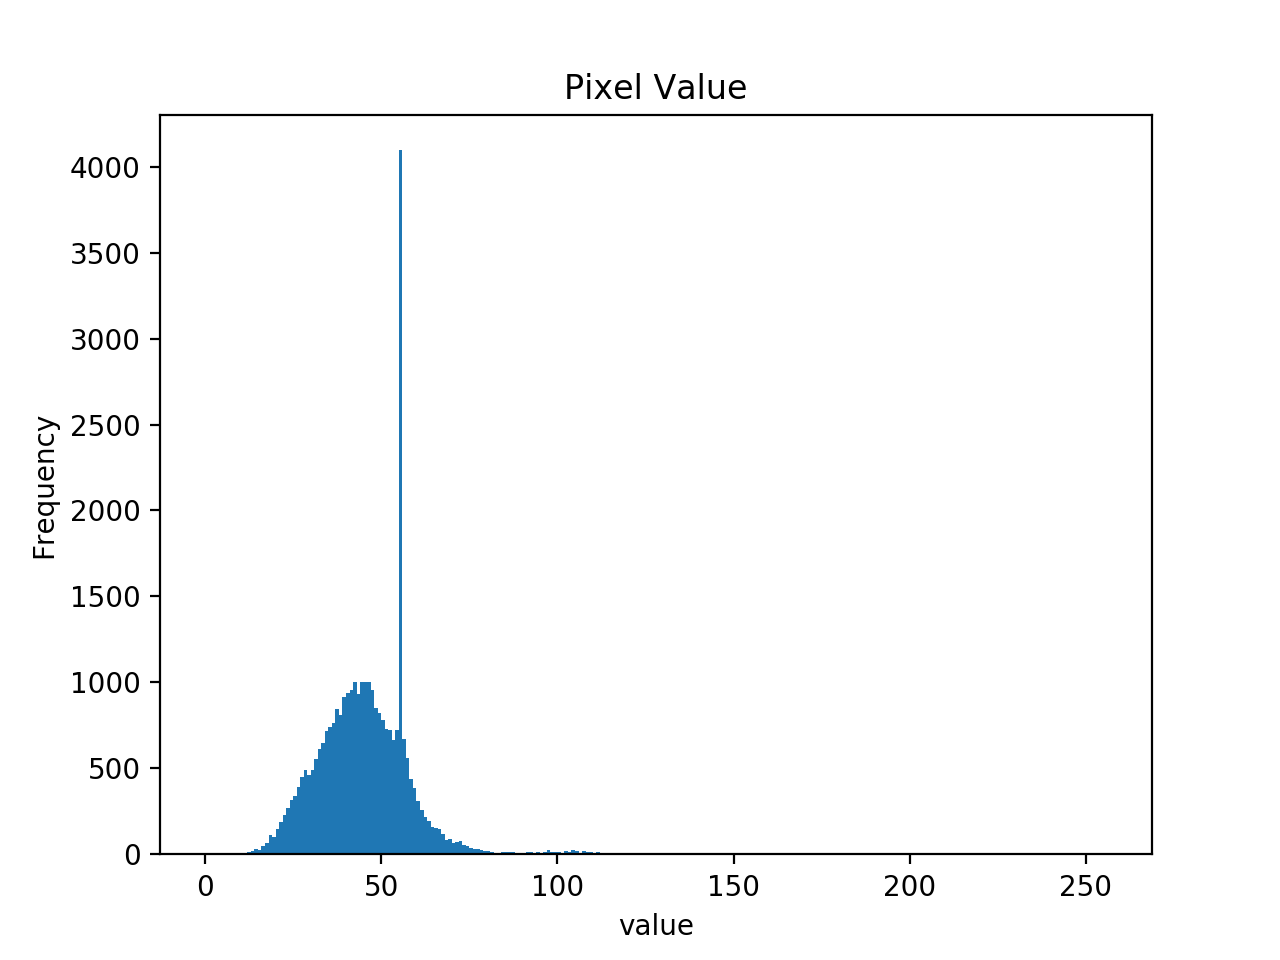
\includegraphics[width=0.7\textwidth]{hist_before.png}
	\caption{The histogram before applying the functions.}
	\label{fig:histBif}
\end{figure}

As the information about the exact approach used in the article is inadequate, an adaptive algorithm is created. The algorithm implemented identifies a threshold value based on the histogram. This is done by first identifying the highest and lowest bin-value, which has a frequency of more than a specified "recognition value", which is set to 10 in this project. The recognition value is introduced to make sure outliers are not defining for the threshold. Afterwards the threshold is calculated by the formula in \autoref{eq:pix_threshold}, where \textit{Fraction} is a parameter set manually defining how large a part of the identified pixel value range has to be thresholded. During the processing in this project \textit{Fraction} is set to be equal to $0.1$. 

\begin{equation}\label{eq:pix_threshold}
	\text{Threshold}=\text{Low~Value}+\text{Fraction}\cdot(\text{High~Value}-\text{Low~Value})
\end{equation}


After the threshold has been found it is applied to all pixels in the image. The pixels lower than the threshold are eliminated and have to be reconstructed from neighbouring pixels. Also here the article provides very limited information about the algorithm applied for reconstruction. Therefore an algorithm was implemented, which restores pixels from non-occluded neighbour pixels. A part of the algorithm identifies the pixels with values lower than the threshold and saves the pixel coordinates of these pixels. The saved pixels are  reconstructed iteratively from neighbouring pixels following the 4-connectivity principle. The pixels are reconstructed when there are at least 2 neighbour pixels they can be reconstructed from. They are only reconstructed from pixels above the threshold, this can be pixels that initially were above the threshold, or it can be pixels that have already been reconstructed. The pixels are reconstructed by assigning the average of the neighbours with values above the threshold as the new pixel value. Once all thresholded pixels have been reconstructed the resulting image is returned.

Because the eliminated pixels are reconstructed only from pixels with a value higher than the threshold there are certain traits that can be expected in the histogram of the reconstructed image. One of the traits is that there is a flatline from 0 to the threshold value. A second trait is that a peak close to the threshold is likely to occur because the eliminated values are reconstructed from neighbours, which are likely to be close to the value of the eliminated pixels. However, the plotted histogram after reconstruction is as shown in \autoref{fig:histSpill}.

\begin{figure}[H]
	\centering
	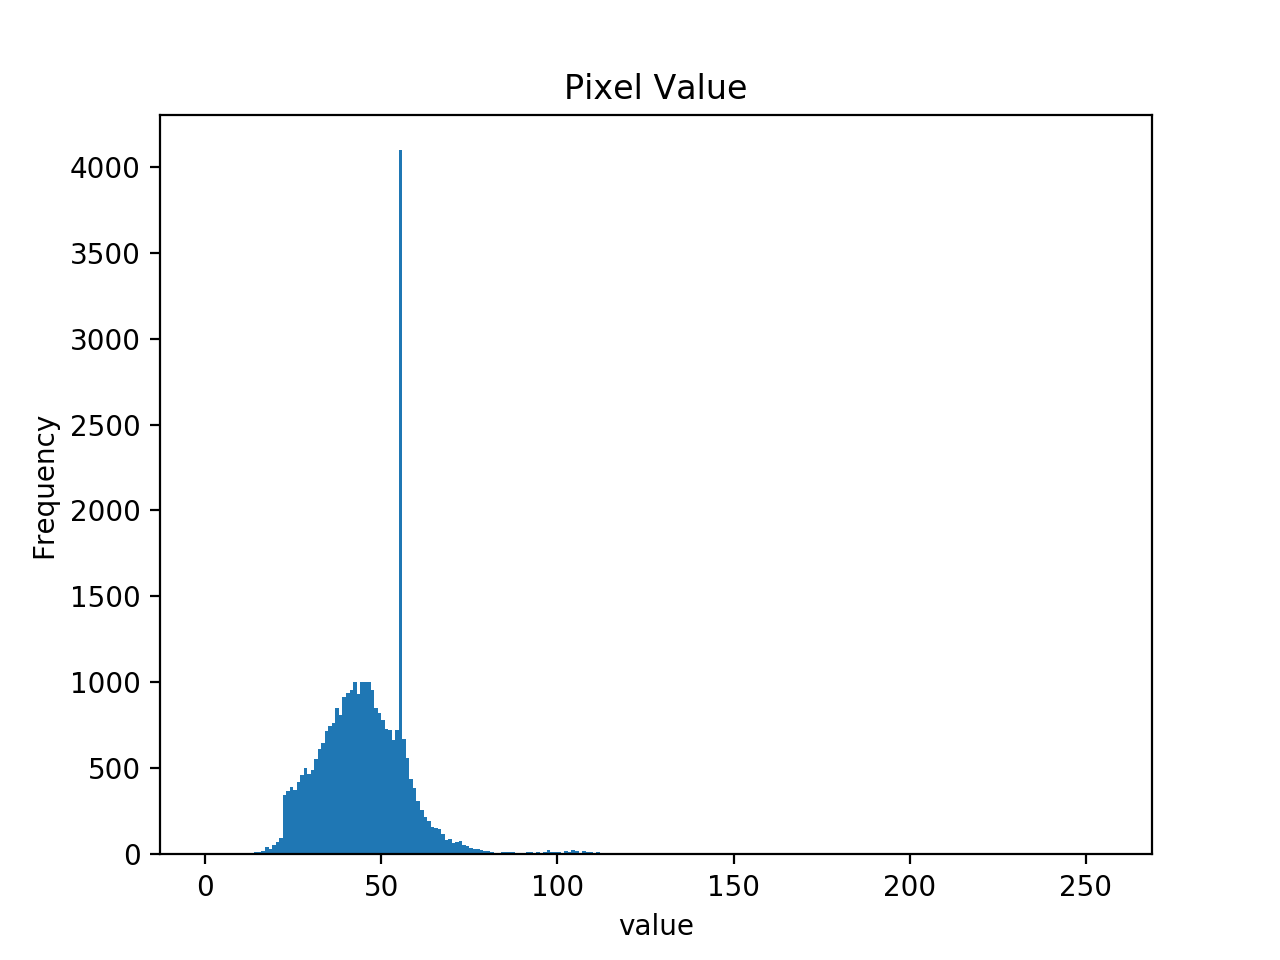
\includegraphics[width=0.7\textwidth]{hist_spill.png}
	\caption{The histogram of the image after reconstruction of pixels.}
	\label{fig:histSpill}
\end{figure}

As can be seen there is a small peak as expected, however, there seem to be a "spill over" across the threshold to the lower values. By closer examination of the code it was discovered that this was caused due to a programming mistake. The mistake was that the values used for reconstruction were obtained from the original image and not from the reconstructed image. Once this mistake was corrected the histogram was as expected as shown in \autoref{fig:histFine}. 

\begin{figure}[H]
	\centering
	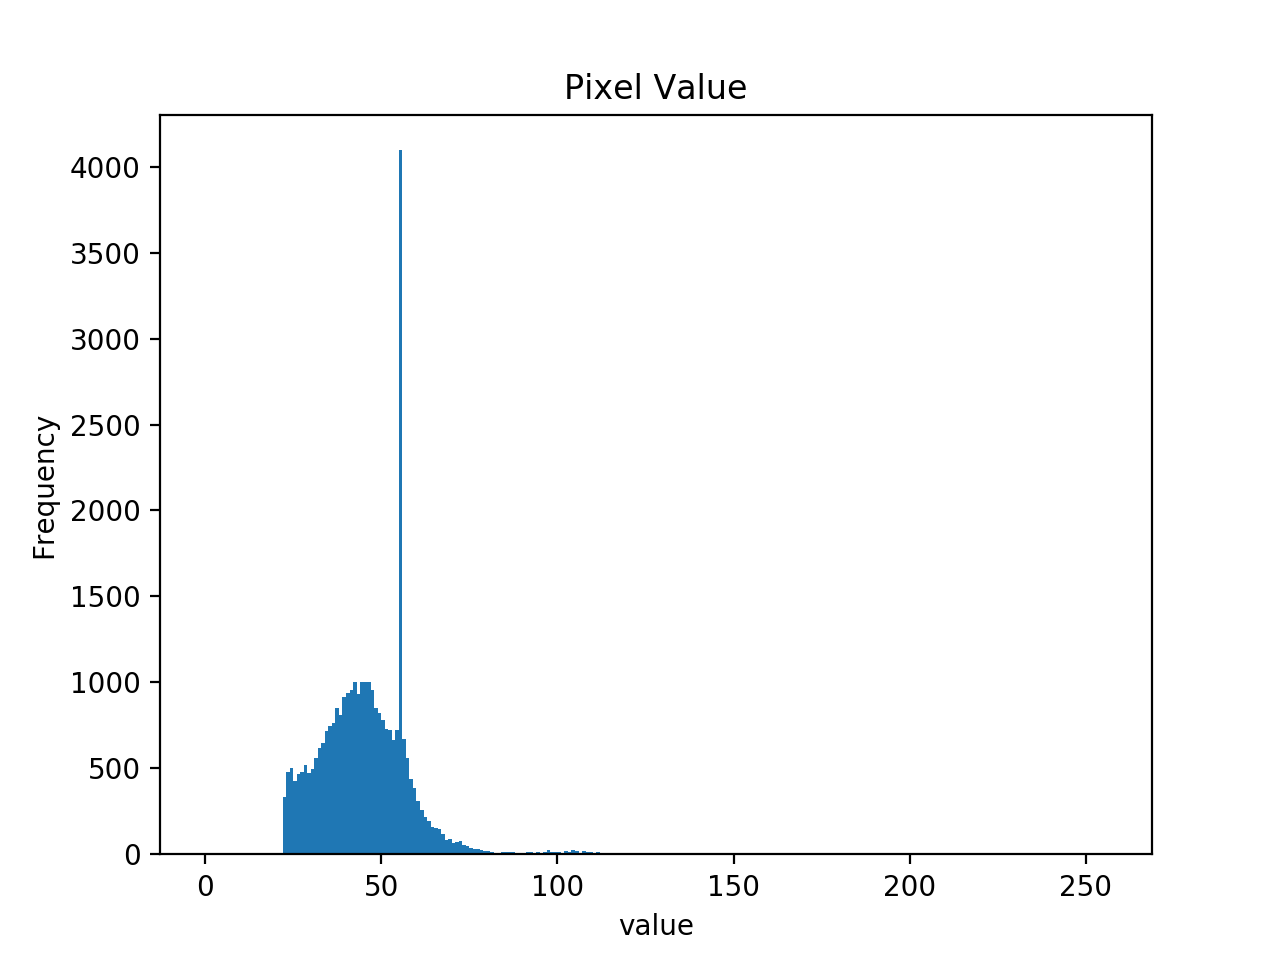
\includegraphics[width=0.7\textwidth]{hist_nicespacing.png}
	\caption{The histogram of the image after applying the corrected noise remover function.}
	\label{fig:histFine}
\end{figure}

In relation to the reconstruction of pixels it should be noted that it could have been done with 8-connectivity, and the iterative process could be split up to more steps, such that pixels are always constructed from as many neighbours as possible. This may give a better reconstruction, however, this has not been investigated. 
Furthermore, small tests showed that the adaptive threshold is difficult to define in an optimal way. If the threshold is too low the eyelash might be reconstructed from edge pixels of the eyelash creating just a lighter eyelash, which is still darker than the iris in the background. If the threshold is higher, it might eliminate the eyelashes, but also be destructive to darker parts of the iris. Maybe this could also be solved if the reconstruction happened based on the neighbourhood and not just the most adjacent neighbour pixels.
 
During implementation the histograms were frequently inspected in order to ensure the results were as expected. \autoref{fig:HistEli} shows a histogram with some eliminated pixel values. It turns out that the function used for generating histograms in python by default takes the range of the pixel values and splits that into as many bins as specified. As a result some of the bins cover a range of values that is entirely between two integer values and thus do not count any instances of pixel values as they are always integers between 0 and 225. This was solved by passing a specific range $[0,256]$ as an argument and then the histogram was as displayed in \autoref{fig:histFine}.

\begin{figure}[H]
	\centering
	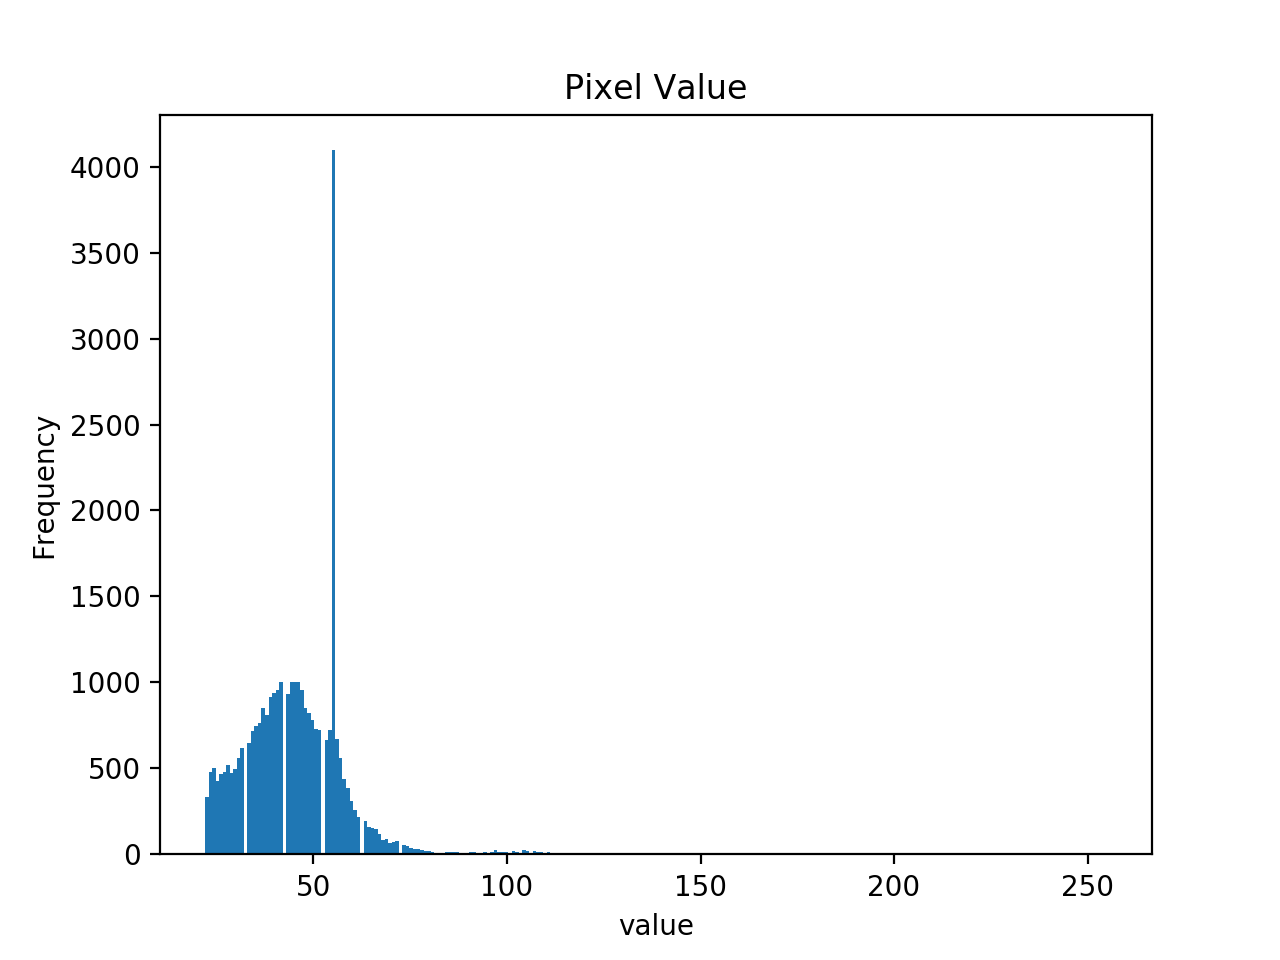
\includegraphics[width=0.7\textwidth]{hist_troublespacing.png}
	\caption{The histogram of the reconstructed image with eliminated values.}
	\label{fig:HistEli}
\end{figure} 

\subsection{Histogram Equalisation}
\label{sec:HistEq}
The histogram equalisation is applied to increase contrast. This is necessary to enhance the structures in the iris. This was implemented manually. As in the noise removal the lowest and highest bin values with more instances than a specified value are found. Based on the values found, the histogram is stretched using the formula in \autoref{eq:hist_stretch}.

\begin{equation}\label{eq:hist_stretch}
	\text{New~Pixel~Value}=(\text{Pixel~Value}-\text{Low~Value})\cdot\frac{255}{\text{High~Value}-\text{Low~Value}}
\end{equation}

The pixels, which have values above $ 255 $ or below $ 0 $ after the formula is applied, are set to $ 255 $ or $ 0 $ respectively. The resulting image is shown in \autoref{fig:irisST}, while \autoref{fig:histST} shows the histogram after applying the formula to each pixel.

\begin{figure}[H]
\centering
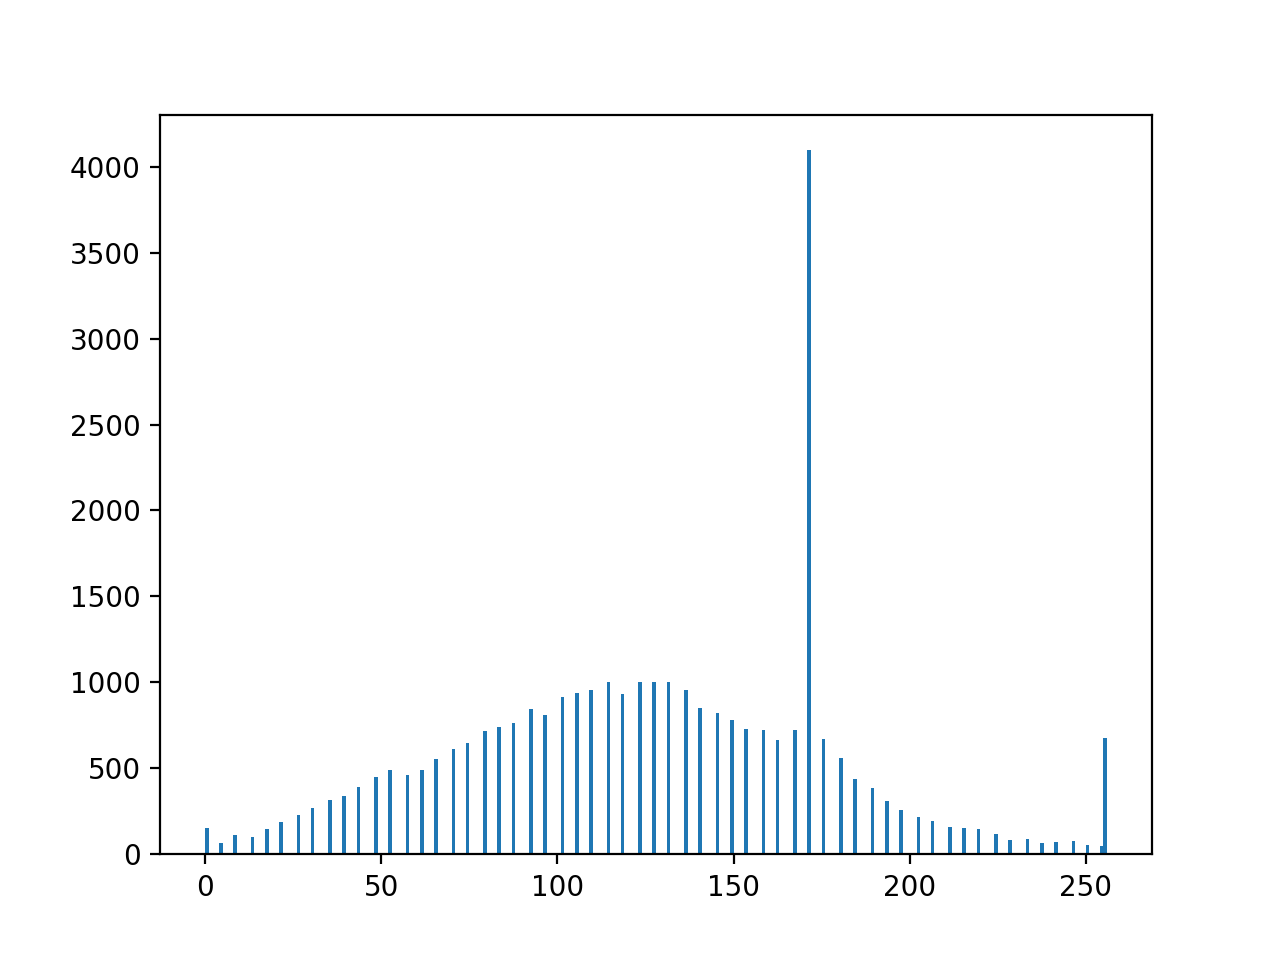
\includegraphics[width=0.7\textwidth]{Stretch_hist.png}
\caption{The histogram of the image after applying the initial "equalise histogram" function.}
\label{fig:histST}
\end{figure}

However, it was discovered that the implemented method was actually histogram stretching, which was mistakenly taken as the same as histogram equalisation. Though the two methods have somewhat the same effects, histogram equalisation is better at ensuring a uniform spreading of the pixels across the histogram. 
This is done by identifying a transform of the bin values which causes the \gls{cdf} of the histogram to be as linear as possible, and apply it to the grey levels or bin values. The result of the histogram equalisation is showed in \autoref{fig:irisEQ} and \autoref{fig:histEQ}.

\begin{figure}[H]
\centering
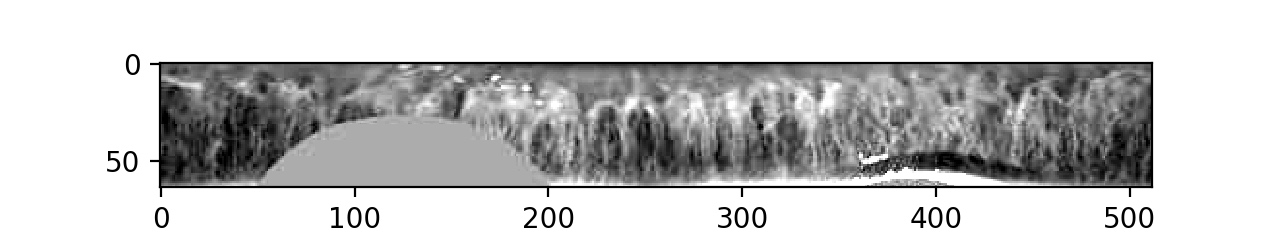
\includegraphics[width=\textwidth]{Stretch_iris.jpg}
\caption{The image of the iris after applying the initial "equalise histogram" function.}
\label{fig:irisST}
\end{figure}
\begin{figure}[H]
\centering
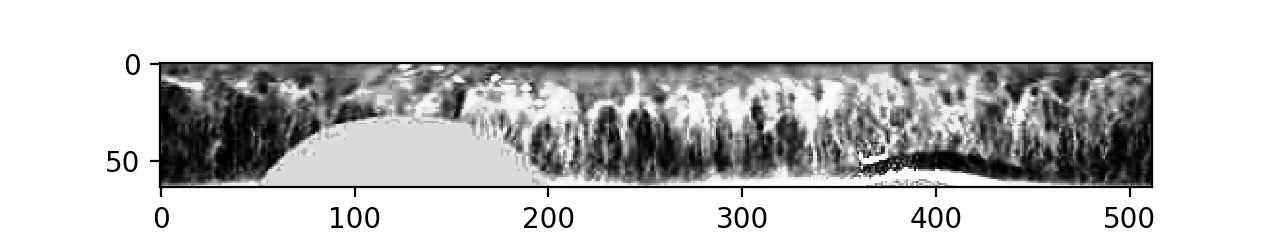
\includegraphics[width=\textwidth]{Equal_iris.jpg}
\caption{The image of the iris after applying the real equalisation of the histogram.}
\label{fig:irisEQ}
\end{figure}
\begin{figure}[h]
\centering
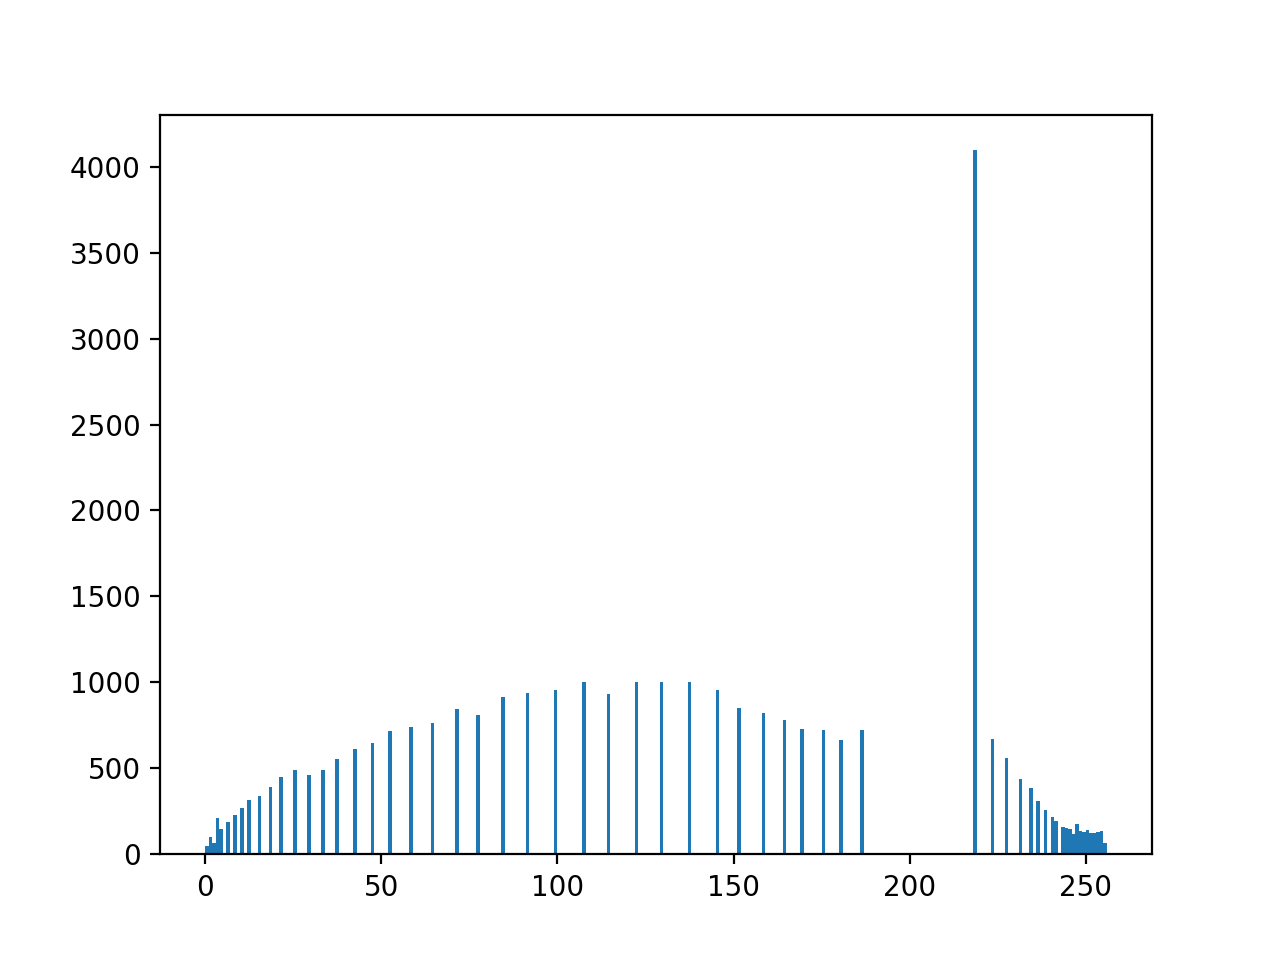
\includegraphics[width=0.7\textwidth]{Equal_hist.png}
\caption{The histogram of the image after applying the real equalisation of the histogram.}
\label{fig:histEQ}
\end{figure}

When comparing the two images of the iris, after applying the two different contrast adjustment methods, it can be concluded that the histogram equalisation does indeed result in better contrast and a more enhanced and out spoken appearance of the structures in the iris than the histogram stretching does. Testing also showed that using the equalisation rather than the stretching increased the accuracy, this is further addressed in \autoref{MachineLearnClassification}. 

\subsection{Feature extraction}
As it is difficult to extract all the complex structures in the iris, the work presented uses the iris image as input. However, because the image in full will result in too large amounts of data to handle during classification, feature extraction is done. Feature vectors are extracted using Haar wavelets in a wavelet decomposition. 
Haar wavelets are a fast and simple way to obtain wavelets. In Haar wavelets, the decomposition is done by calculating the average of neighbouring pixels as well as half the difference between neighbouring pixels. Due to the way the method works the image is lowpass or hi-pass filtered two times in each of the possible combinations. The image of the greatest interest in this case is the one that has been lowpass filtered in both horizontal and vertical direction, this is referred to as LL. This image will be a compressed version of the original image, showing an approximation or the tendency of the original image. The other images created in one stage are HH, HL, LH all of which contain detail coefficients. HH is representing the diagonal detail, while HL presents horizontal detail and LH presents vertical detail. The LL will naturally appear in the upper left corner of the output matrix. 

In order to compress the image sufficiently three stages or passes of Haar wavelet decomposition was carried out. The result is shown in \autoref{fig:haar3}. 

\begin{figure}[H]
\centering
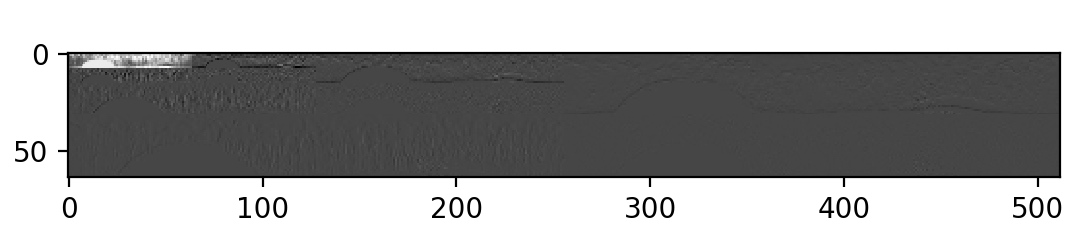
\includegraphics[width=\textwidth]{haar_3.jpg}
\caption{The result of the three level Haar wavelet decomposition. Note that the small light image in the upper left corner is the LL3, which is used onwards.}
\label{fig:haar3}
\end{figure}
The resulting matrix of LL3 coefficients is then put into a feature vector, which is used for training the classifiers described in \autoref{MachineLearnClassification}.

\subsection{Training and Classification}
\label{MachineLearnClassification}
In the work described in the article different classifiers were tested. The best of the investigated classifiers are the \gls{knn}, \gls{lda}, as well as \gls{svm} with linear or quadratic kernel. In the following sections the theory behind the different classifiers is briefly described.

\subsubsection*{K-Nearest Neighbour}
\gls{knn} is one of the most simple supervised classification methods. It is a non-parametric method. This means that the training data is used "raw" and there are no parameters that are deducted from the data in order to form a model. 
 
\gls{knn} utilises Bayes' theorem in order to determine the probability of a sample belonging to a certain class. The probability of the sample belonging to different classes is found by examining the density of datapoints belonging to the different classes among the $k$ nearest neighbours. The probability of a class given the sample can be estimated by the formula in \autoref{eq:classProb}.

 \begin{equation}\label{eq:classProb}
	p(C_k|\text{x})=\frac{K_k}{K}
\end{equation}

Where $C_k$ is a given class, $\text{x}$ is the sample, $K$ is the number of neighbours considered, and $K_k$ is the amount of data points among the $K$ neighbours belonging to the class $C_k$.

Finally, a class is assigned to the sample based on which class has the highest conditional probability.

The value $K$ greatly influences the way the classifier performs. Therefore it is important to determine an optimal value of $K$. This may depend on the performance but also the amount of data that has to be compared with. In this project $K$ is found by determining which value of $K$ for $K\in[1,30]$ results in the best performance. This is done by training on a test set of five images and evaluating the train error. \autoref{fig:misclassK} shows the misclassification error dependent on the value of $K$. As seen in the figure $K=1$ results in the lowest misclassification error, therefore this is used going forth in the project work.  
 \begin{figure}[H]
\centering
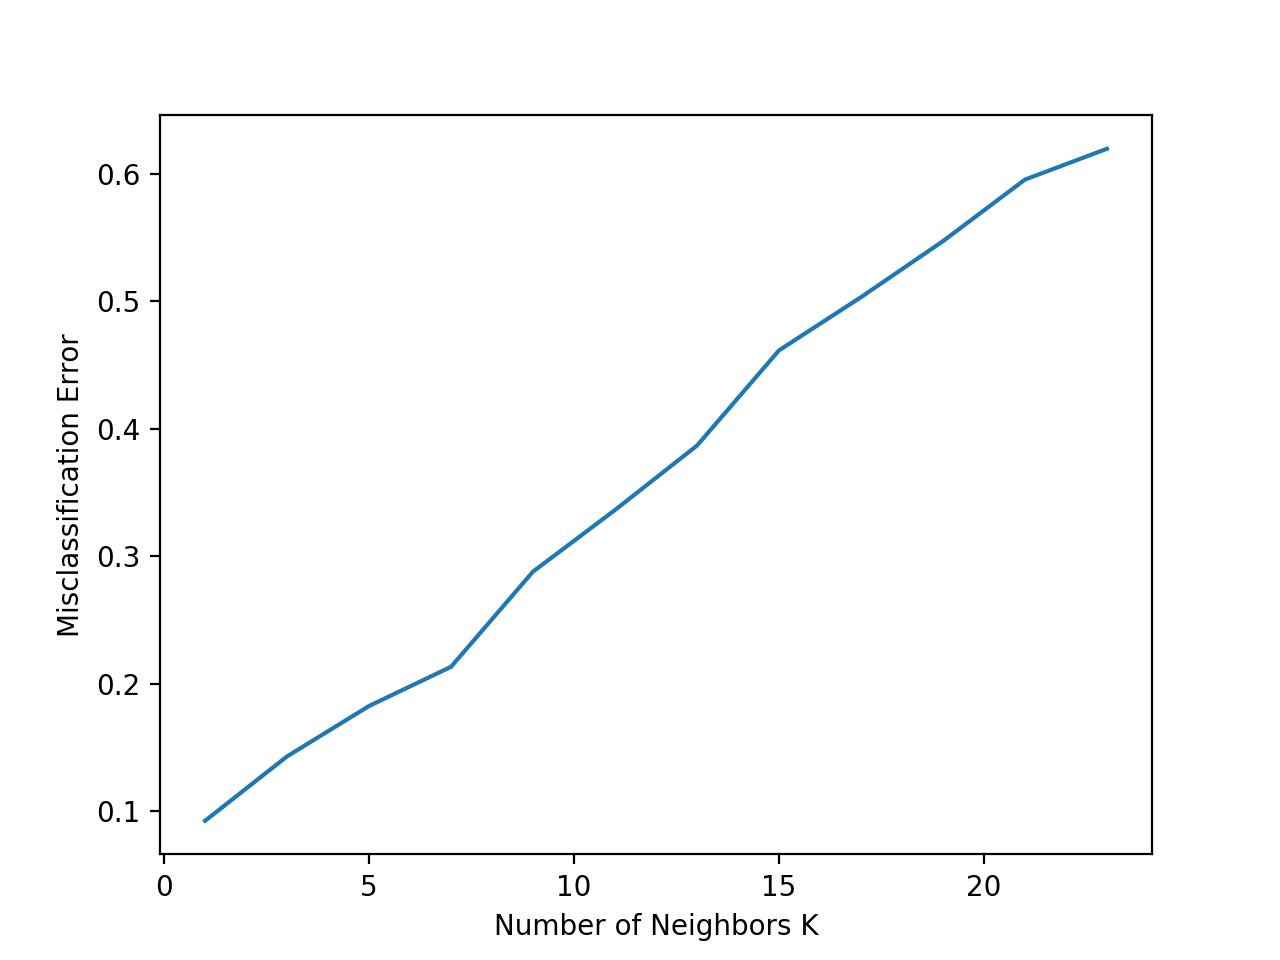
\includegraphics[width=0.8\textwidth]{kgraph.png}
\caption{The misclassification error for the \gls{knn} as a result of the number of neighbours $K$ used for the classifier.}
\label{fig:misclassK}
\end{figure}
\subsubsection*{Linear Discriminant Analysis}
\gls{lda} is a parametric method, which is trained by supervised learning. \gls{lda} is a classifier in which linear decision boundaries are learned based on training data. It is part of a more general group of linear discriminant functions. The decision boundary is found such that interclass variance is maximised while intra class variance is minimised. There are a range of possibilities for identifying the equation for the linear decision border eg. by using SVD or EVD.    

\subsubsection*{Support Vector Machines}
\gls{svm} identifies the optimal linear hyperplane as the decision boundary. The decision borders are found for linearly separable data. A separating hyperplane is not necessarily unique, however, the optimal hyperplane should be unique. The optimal linear decision boundary is found by identifying the hyperplane, which has the maximal margin around it not intersecting with any data points in the training set.
In practice the hyperplane is found based on a subset of data points that lie close to the separating plane, those are called the support vectors.    

However, in some cases the data is not linearly separable. For those cases Kernel Functions can be applied before identifying the optimal hyperplane. The kernel function maps the original data from the original space into a new space, where it can be linearly separated.  

\subsubsection*{Cross Validation}
In this project the above mentioned classification methods are implemented. Just as in the work described in the article, cross validation is carried out in order to test the performance of the classifiers. Five images per class are used for the cross validation. The cross validation done is a five fold cross validation. However, since some classes have too few images those classes are neglected. As mentioned in \autoref{sec:HistEq} changing from histogram stretching to histogram equalisation affects the performance of the classifiers. In \autoref{tab:fiveFoldClas} the accuracies as well as the precision of the classifiers in both the case with histogram stretching and histogram equalisation are shown.  

\begin{table}[H]
\centering
\begin{tabular}{|l|c|c|c|c|}
\cline{2-5}
\multicolumn{1}{c|}{}&\multicolumn{2}{c|}{Histogram Stretching}&\multicolumn{2}{c|}{Histogram Equalisation}\\
\hline
Classifier&MA (\%)&$2\sigma$ (\%)&MA (\%)&$2\sigma$ (\%)\\
\hline
KNN (k=1)&$79$&$\pm 6$&$91$&$\pm4$\\
\hline
LDA&$94$&$\pm2$&$95$&$\pm3$\\
\hline
SVM (Linear)&$85$&$\pm8$&$92$&$\pm2$\\
\hline
SVM (quadratic)&$77$&$\pm8$&$92$&$\pm4$\\
\hline
\end{tabular}
\caption{Performance of the different classifiers evaluated by five-fold cross validation. MA is for Mean Accuracy, and $\sigma$ is the standard deviation}
\label{tab:fiveFoldClas}
\end{table} 
Considering the results for the \gls{knn} and the quadratic \gls{svm} shown in \autoref{tab:fiveFoldClas} there seems to be a significant increase in the accuracy of the two classifiers. However, since it is based on such a limited amount of measurements it is probably more representative and valuable to consider the general trends. When comparing the two accuracies across all of the classifiers there seems to be evidence for an increase in accuracy when the histogram equalisation is used rather than the histogram stretching. Therefore the histogram equalisation is used from this point on. 
\begin{table}[H]
\centering
\begin{tabular}{|l|c|c|c|}
\cline{2-4}
\multicolumn{1}{c|}{}&\multicolumn{3}{c|}{Cross Validation Accuracy (\%)}\\
\cline{2-4}
\multicolumn{1}{c|}{}&\cite{Khan2017a}&\multicolumn{2}{c|}{Replicated}\\
\hline
KNN (k=1)&95.1&91&91\\
\hline
LDA&94.28&94&\textbf{95}\\
\hline
SVM (Linear)&96.46&91&92\\
\hline
SVM (quadratic)&\textbf{97}&92&92\\
\hline
\end{tabular}
\caption{Comparison of the performance of the different classifiers achieved by \cite{Khan2017a} and the replicating work in this project. The first column under "Replicated" are accuracies based on data from 55 classes, while the second column is based on data from 91 classes.}
\label{tab:fiveFoldClasCompare}
\end{table} 

In \autoref{tab:fiveFoldClasCompare} the accuracies achieved by the work of \cite{Khan2017a} are compared with the accuracies achieved in the replication of the work when conducting five-fold cross-validation on a set of 5 images from each class. The comparison reveals that the replication does not achieve the same accuracies. In general the original work seems to acquire higher accuracies, however, the original work does not present the variance of the mean accuracy calculated in relation to the cross validation. Therefore, it is impossible to verify how precise the classifiers in the original work are. Another thing to note is the fact that the quadratic \gls{svm} is the one that performs best according to the original work, while the replicated work suggests that the \gls{lda} classifier gives the highest accuracy. There are several factors that might contribute to the difference between the results presented in the original work and the result obtained through replication. One factor might be the amount of data. Though the amount of data samples used per class is the same, the amount of classes is not the same. Due to some issues with processing of the database, which are described in \autoref{sec:ChallDatabase}, only a part of the database was available for testing. First only 55 classes were available and after a while 91 classes of the total 140 classes in the database. Some tests were done with both 55 and 91 classes and the results show that the amount of classes does influence the accuracies as is shown in \autoref{tab:fiveFoldClasCompare}. Another factor that might cause different results is the fact that some steps of the processing are described quite briefly, thus the replication of the work might not be entirely aligned with the original work. 

\begin{table}[H]
\centering
\begin{tabular}{|l|c|c|c|}
\cline{2-4}
\multicolumn{1}{c|}{}&\multicolumn{3}{c|}{Classification accuracy (\%)}\\
\hline
Classifier&Train&Test&Validation\\
\hline
KNN (k=1)&100&96&97\\
\hline
LDA&100&98&97\\
\hline
SVM (Linear)&100&97&98\\
\hline
SVM (quadratic)&100&98&98\\
\hline
\end{tabular}
\caption{The different accuracies achieved by the classifiers when trained on 70\% of the data and tested and validated respectively on 15\% of the data.}
\label{tab:ClasAccMachine}
\end{table} 

In order to examine the performance of the systems implemented in this work when trained on more data a test was conducted. During the test the classifiers were trained on 70\% of the data and were tested on 15\% of the data. Finally they were validated by testing on the remaining 15\% of the data. The results are shown in \autoref{tab:ClasAccMachine}. As the table shows the train accuracies for all the classifiers are 100\%, which means the models are fitted perfectly to the train data. As can be expected, the test and validation accuracies are lower than the train accuracy. It is worth noting that the accuracies are higher than the accuracies obtained in the cross validation based on only a smaller amount of data. Furthermore, the training on more data results in accuracies higher than the ones obtained in cross validation in the original work. However, this test seemingly confirms the statement of the original work that the quadratic \gls{svm} performs best.

Though the achieved accuracies are quite high, the performance of these machine learning methods still cannot compete with the state of the art accuracies within iris classification and general biometric identification methods as described in \autoref{ch:req}. Therefore, another method, deep learning, is investigated for iris classification in order to explore, whether, this method can classify with accuracies comparable to the state of the art performances and comply with the requirement of an accuracy higher than 99\%. The work on the implementation of a \gls{cnn} for iris classification is described in \autoref{sec:cnn_iris_rec}.

\subsection{Challenges}
\label{sec:ChallDatabase}
As mentioned previously several issues were encountered during the implementation of the work described in this chapter. This section elaborates on a few of the issues. 

\subsubsection{Algorithm Description} 
Although overall steps of the processing algorithm are presented in the article by \cite{Khan2017a}, there are a lot of unclear details when considering the descriptions of the individual steps of the processing. This makes it difficult to replicate the work conducted in the article, and it results in parts of the code being implemented based on the best knowledge supplemented with ideas, while other things are based on the indications from tests.

\subsubsection{Processing Issues}
Once the algorithm was implemented it had to be applied in order to process the entire Warsaw-Biobase database consisting of 3192 images of irises obtained from 70 subjects used as 140 classes. The handling and processing of this amount of data proved quite troublesome. First of all, the processing of one image using the implemented MATLAB libraries takes quite some time. The time of course depends on the resources of the computer, however, it took a few minutes per image. Furthermore, the process sometimes reported that it was too demanding for the laptops used. Therefore, the processing was moved to be carried out by a desktop PC with more computational power. This was a shared computer borrowed through an internet connection using TeamViewer, which meant that it was only accessible sometimes. 

Another issue was the variation in the images being processed. Though the algorithm is implemented in a way that is somewhat flexible, which automatically identifies the areas of interest, it does sometimes fail. In some cases the algorithm is unable to identify the wanted area or it falsely identifies the wrong area as the area of interest. In those cases the algorithm would break or get stuck, which required manual restart or continuation of the processing. 

The combination of the algorithm not running continuously, and the fact that accessing the running processing was only possible sometimes, made it difficult to ensure that the algorithm was running, and as a result the process would waste large amounts of time being stuck on a single image. Therefore, processing of the full database was not completed, however, 2086 images in 91 classes of the full 140 classes were processed and used for the development and testing in the project work. 











%\graphicspath{{figures/test/}}
\chapter{Tests}

%\chapter{Conclusion}\label{ch:conclusion}\glsresetall
Throughout the project, the work has been aimed at finding a solution to the problem statement; \\
\textbf{How well can identity verification be performed on \gls{vl} smart phone images of iris and face, and to which extend can the performance be improved by information fusion?}

To be able to perform identity verification on smart phone images of iris and face, several recognition solutions was made.

Iris recognition was done in multiple ways. Firstly, different regular machine learning solutions was made. The best performance was using a polynomial kernel for \gls{svm}, with an accuracy of $98\%$ which did not meet the requirement set for the accuracy.
Therefore, a deep learning solution was introduced. By using a \gls{cnn} with a total of 14 layers, it was possible to achieve an accuracy of $99.7\%$, which satisfied the requirement of at least $99\%$ accuracy. 
Both the machine learning and deep learning solution used the Warsaw BioBase database, a database with close-up photos of irises captured with an Apple iPhone 5s.

Face recognition was made using a pre-made image classification model, VGG16. This model is pre-trained on the ImageNet database with 2000 different classes, and the weights from this are used in the implementation of the model. The \gls{cnn} used the \gls{lfw} database and achieved an accuracy of $99.35\%$, which also satisfied the requirement of accuracy limit.

A fusion of the two successful \gls{cnn}s was then made. For this network, the databases used with the two separate networks was combined into one database with a label for an iris and a face tying them together. This network achieved an accuracy of $81.17\%$, which is not better than any of the stand-alone networks.

% For use if report is split up in parts
\bookmarksetup{startatroot}% Goto root of Table of Contents
\addtocontents{toc}{\bigskip}% Add space before next item in Table of Contents

% Appearance of the bibliography
\iflanguage{english}{%
\bibliographystyle{setup/plainnat_en}%
}{%
\bibliographystyle{setup/plainnat_dk}%
}
\label{LastPage}


\bibliography{bib/VGIS8.bib}
\label{bib:mybiblio}




%\setlength{\chapnumb}{2cm} % Ændrer længden på stregen under kapiteloverskriften så den passer til bilag
\appendix % Start of appendix
\addtocontents{toc}{\protect\setcounter{tocdepth}{0}} 


\end{document}
